\documentclass[10pt]{article}
\usepackage[margin=0.8in]{geometry}
\usepackage{graphicx,booktabs,float,hyperref,xcolor,amsmath,caption}
\captionsetup{font=small}
\hypersetup{colorlinks=true,linkcolor=blue,urlcolor=blue}
\title{SAGE-Extend 3D: pipeline repair, geometry-aware knowledge-grounded editing,\\ and a controlled pilot (interim technical report)}
\author{SAGE-Extend 3D project (generated from repository artifacts)}
\date{2026-10-14 15:51}
\begin{document}
\maketitle
\noindent\fcolorbox{red!60!black}{red!4}{\parbox{0.97\linewidth}{\small
\textbf{Read first.} Only the input photographs are real. Every 3D asset and every rendered view is \emph{synthetic}. SAGE contains a single view per specimen, so \textbf{no novel view, hidden structure or 3D shape is verified against reality}. Biological plausibility was \textbf{not} assessed by experts (none available). All numbers come from a 15-specimen pilot on a local 2$\times$TITAN X machine. Effects are reported with confidence intervals; nothing is claimed significant unless stated.}}
\section*{Summary}
\begin{itemize}
\item \textbf{Reconstruction.} The low input-view IoU reported in the interim was a SAM~3D pose/scale error (objects over-scaled in 13/15), not a camera error. A pose-only correction raises median IoU from 0.63 to 0.92 on all 15 reconstructions. This is a fit to the input silhouette, not an accuracy measurement. One specimen (Peach 0006) is a reconstruction failure.
\item \textbf{Arm F} failed only because of prompt serialisation (fixed and verified on live runs). A second bug (non-finite opacity $\rightarrow$ NaN $\rightarrow$ every fp16 step skipped) explained the ``no change'' on Peach 0006.
\item \textbf{GaussianEditor does not edit geometry.} Its Gaussians move incoherently (displacement coherence 0.31 vs 0.25 for noise); the sheet thickens and the texture becomes grainy. KB text changes its colour output but not its geometry: F vs E coherence 0.31 vs 0.31 ($\Delta$ +0.00, specimen-bootstrap 95\% CI [+0.00, +0.00], 11/15 specimens favour the first arm, 5 classes).
\item \textbf{A KB-driven geometry editor} produces coherent, measurable deformation (coherence $\approx$1). Against an equal-magnitude generic warp, KB geometric recall is 0.44 vs 0.07 ($\Delta$ +0.37, specimen-bootstrap 95\% CI [+0.13, +0.61], 4/6 specimens favour the first arm, 2 classes). Recall is partly by construction; biological correctness is unvalidated.
\item \textbf{Cross-view consistency} (same surface point, adjacent views, median $\Delta$E): per-view 2D edits 16.8/19.3 (generic/KB), GaussianEditor 3D 9.3, geometry-only 3D 2.0, against a floor of 2.0. This is internal consistency only.
\item \textbf{Not established:} external validity of any novel view (no reference data), biological validity (no experts) and downstream utility (not run).
\end{itemize}

\section{Data, scope and provenance}
All inputs are single real photographs from SAGE (HF \texttt{tirtho149/SAGE}, CC-BY-4.0), from the leakage-safe \emph{build} split (SHA-1 dedup, pHash clusters, grouped splits; \texttt{reports/phase1\_protocol/02\_dataset\_protocol.md}). Fifteen pilot specimens span five classes: Peach Leaf Curl, Tomato Leaf Mold, Corn Smut, Citrus Canker and Mango Anthracnose (negative control). \textbf{No second real view or 3D measurement of any specimen exists.} By user decision, no external multi-view dataset was used. Every rendered view of a 3D asset is therefore \emph{synthetic and unverified}. Expert review was not available. All runs used the local machine (2$\times$ GTX TITAN X, 12\,GB, Maxwell); Nova/Slurm were not used.

\section{Methods}
\paragraph{Reconstruction and alignment.} SAM~3D Objects (stage-wise CPU/GPU offload; locally reproduces the A100 output to a Chamfer distance of $4.5\times10^{-5}$ of the bbox diagonal). Input-view alignment study A0--A3: A0 is the existing pose; A1 tests the camera convention; A2 is a closed-form scale and translation; A3 is a 7-DoF render-and-compare of the object pose with geometry frozen and a mask-only loss. The corrected pose is A3* = A3 if it beats A2, otherwise A2. LPIPS and MoGe depth agreement are held out.
\paragraph{GaussianEditor diagnosis.} Code inspection plus per-Gaussian before/after comparison, using prune-aware index correspondence (verified bit-exact on a no-op run): displacement, k-NN displacement coherence (1 = smooth field, 0.25 = i.i.d.\ noise), rotation, scale, opacity, colour, sheet thickness.
\paragraph{Geometry editor (G2).} Edited positions $\mu_i'=\mu_i+m_i d_i$, with $d$ minimising
$\lambda_1\,\mathrm{mean}_i\, m_i(d_i\!\cdot\! n_i-h_i)^2/L^2+\lambda_2\,\mathrm{mean}_{ij}\big((\|e'_{ij}\|-\|e_{ij}\|)/\|e_{ij}\|\big)^2+\lambda_3\,\mathrm{mean}_{ij}\|m_id_i-m_jd_j\|^2/L^2+\lambda_4\,\mathrm{mean}_i(1-m_i)\|d_i\|^2/L^2$,
with $(\lambda_1..\lambda_4)=(1,0.1,0.01,1)$ over an 8-NN graph. $L$ is the bbox diagonal, so all quantities are unit-free. The target normal offset $h$ is built from KB operators: \emph{pucker} (zero-mean Poisson-disk blisters), \emph{distort} (low-frequency warp), \emph{thicken} (Gaussian scale along the normal), \emph{outgrowth} (galls), \emph{depress} (pits). Rotations follow the change of the local normal. Colours and opacities are untouched. The generic control G uses a random smooth vector field of equal RMS.
\paragraph{Structured KB grounding.} Only the verbatim web quote is evidence. It is split into stages at temporal markers, and one stage is edited. Prompts are a fixed template plus verbatim phrases (asserted in code). Hedged phrases are excluded and other-stage features are prohibited. Terms without an operator (curl, roll, wilt, corky) are recorded, never approximated.
\paragraph{Arms.} A real; B generic 2D; C KB 2D (interim mixed-stage prompt); C-NG KB without geometry; C-MM mismatched KB; C-stage stage-consistent KB 2D; I 2D shape-capable (mask dilated 15\,\%, image guidance 1.2); Bmv/Cmv independent per-view 2D edits of the ring renders (object-masked); D unedited 3D; E/F GaussianEditor generic/KB (interim settings); G generic geometry; J KB geometry; K GaussianEditor appearance-only with geometry frozen; H = J then K. GaussianEditor prompts are passed through validated per-run configs and checked against GaussianEditor's own parsed config after the run.
\paragraph{Metrics.} Geometry: displacement and coherence; band-split out-of-plane attributes (distortion, blister density, normal thickening, outgrowth; the depression detector proved non-specific and is excluded from recall). Thresholds come from a uniform midpoint rule on a synthetic flat sheet; the operator$\times$detector matrix is diagonal. KB recall is the fraction of the stage's required geometric attributes detected; the unsupported rate is the fraction of detected attributes not called for by the KB. Appearance: CIELAB term detectors with an a-priori threshold of 5 units. Render QC: silhouette and depth change, grain, edge fuzz. Cross-view: same-surface-point $\Delta$E between adjacent views (depth-tested projections), with the unedited asset as the floor. Statistics: the specimen is the unit (seeds averaged); paired cluster bootstrap over disease classes, Wilcoxon, Holm.

\section{Results}\label{sec:res}
\begin{figure}[H]\centering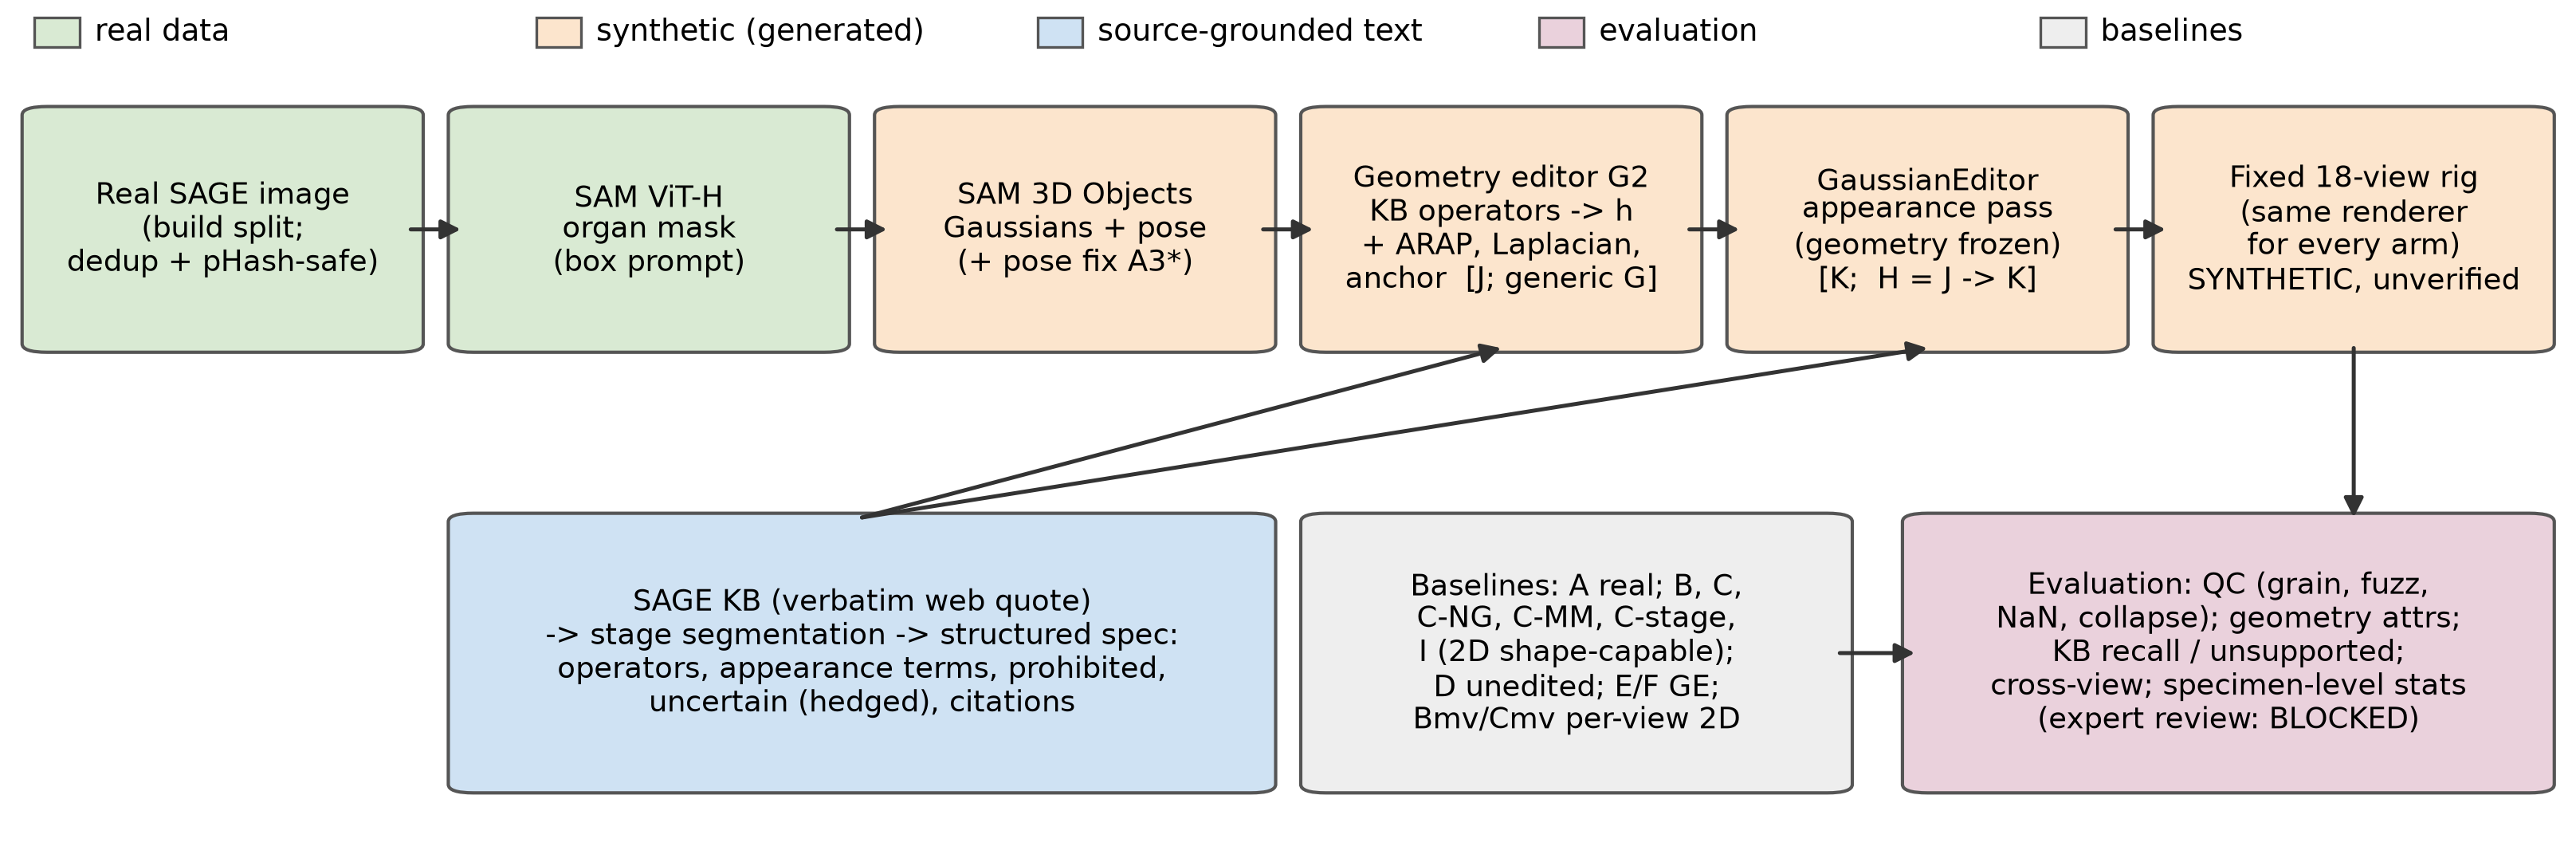
\includegraphics[width=\linewidth]{figs/fig1_pipeline.png}\caption{Pipeline and data status.}\end{figure}

\subsection{Input-view alignment (E1)}
\begin{table}[H]\centering\scriptsize
\caption{E1 input-view alignment (IoU). A1 = principal point at centre; A2 = closed-form scale+translation; A3 = 7-DoF render-and-compare (mask loss only, geometry frozen); A3* = A3 if better than A2. $^\dagger$ diverged. LPIPS and depth agreement with MoGe are never optimised.}
\resizebox{\linewidth}{!}{
\begin{tabular}{lrrrrrrrrrr}\toprule
Specimen & K px & A0 & A1 & A2 & A3 & A3* & area err & LPIPS (held-out) & depth err (held-out) & label \\ \midrule
Citrus Canker 0004 & 0.6 & 0.67 & 0.67 & 0.84 & 0.91 & \textbf{0.91} & 0.44 & 0.29$\to$0.30 & 0.025$\to$0.079 & ok \\
Citrus Canker 0012 & 0.3 & 0.73 & 0.73 & 0.98 & 0.99 & \textbf{0.99} & 0.36 & 0.23$\to$0.21 & 0.095$\to$0.029 & ok \\
Citrus Canker 0016 & 5.6 & 0.76 & 0.77 & 0.98 & 0.98 & \textbf{0.98} & -0.19 & 0.18$\to$0.19 & 0.088$\to$0.071 & ok \\
Corn Smut 0012 & 0.4 & 0.63 & 0.63 & 0.86 & 0.94 & \textbf{0.94} & 0.43 & 0.20$\to$0.18 & 0.011$\to$0.015 & ok \\
Corn Smut 0025 & 4.3 & 0.61 & 0.61 & 0.77 & 0.76 & \textbf{0.77} & -0.09 & 0.22$\to$0.21 & 0.039$\to$0.042 & ok \\
Corn Smut 0052 & 1.0 & 0.72 & 0.72 & 0.83 & 0.90 & \textbf{0.90} & 0.34 & 0.16$\to$0.16 & 0.051$\to$0.091 & ok \\
Mango Anthracnose 0044 & 0.2 & 0.70 & 0.70 & 0.87 & 0.93 & \textbf{0.93} & 0.27 & 0.14$\to$0.12 & 0.009$\to$0.081 & ok \\
Mango Anthracnose 0049 & 0.3 & 0.77 & 0.78 & 0.85 & 0.95 & \textbf{0.95} & 0.19 & 0.11$\to$0.10 & 0.016$\to$0.039 & ok \\
Mango Anthracnose 0094 & 0.3 & 0.63 & 0.63 & 0.82 & 0.86 & \textbf{0.86} & 0.57 & 0.09$\to$0.13 & 0.035$\to$0.060 & ok \\
Peach Leaf\_Curl 0006 & 1.6 & 0.43 & 0.43 & 0.50 & 0.13$^\dagger$ & \textbf{0.50} & 0.68 & 0.18$\to$0.20 & 0.031$\to$0.027 & reconstruction\_failure \\
Peach Leaf\_Curl 0063 & 6.4 & 0.58 & 0.58 & 0.67 & 0.00$^\dagger$ & \textbf{0.67} & 0.35 & 0.11$\to$0.11 & 0.015$\to$0.014 & ok \\
Peach Leaf\_Curl 0087 & 1.6 & 0.84 & 0.85 & 0.89 & 0.95 & \textbf{0.95} & 0.08 & 0.05$\to$0.04 & 0.003$\to$0.012 & ok \\
Tomato Leaf\_Mold 0015 & 0.3 & 0.40 & 0.40 & 0.88 & 0.94 & \textbf{0.94} & 1.50 & 0.20$\to$0.21 & 0.017$\to$0.031 & ok \\
Tomato Leaf\_Mold 0052 & 0.4 & 0.55 & 0.55 & 0.72 & 0.92 & \textbf{0.92} & 0.79 & 0.29$\to$0.28 & 0.034$\to$0.043 & ok \\
Tomato Leaf\_Mold 0092 & 0.5 & 0.47 & 0.47 & 0.84 & 0.23$^\dagger$ & \textbf{0.84} & 1.11 & 0.32$\to$0.32 & 0.030$\to$0.028 & ok \\
\bottomrule\end{tabular}}\end{table}


\begin{figure}[H]\centering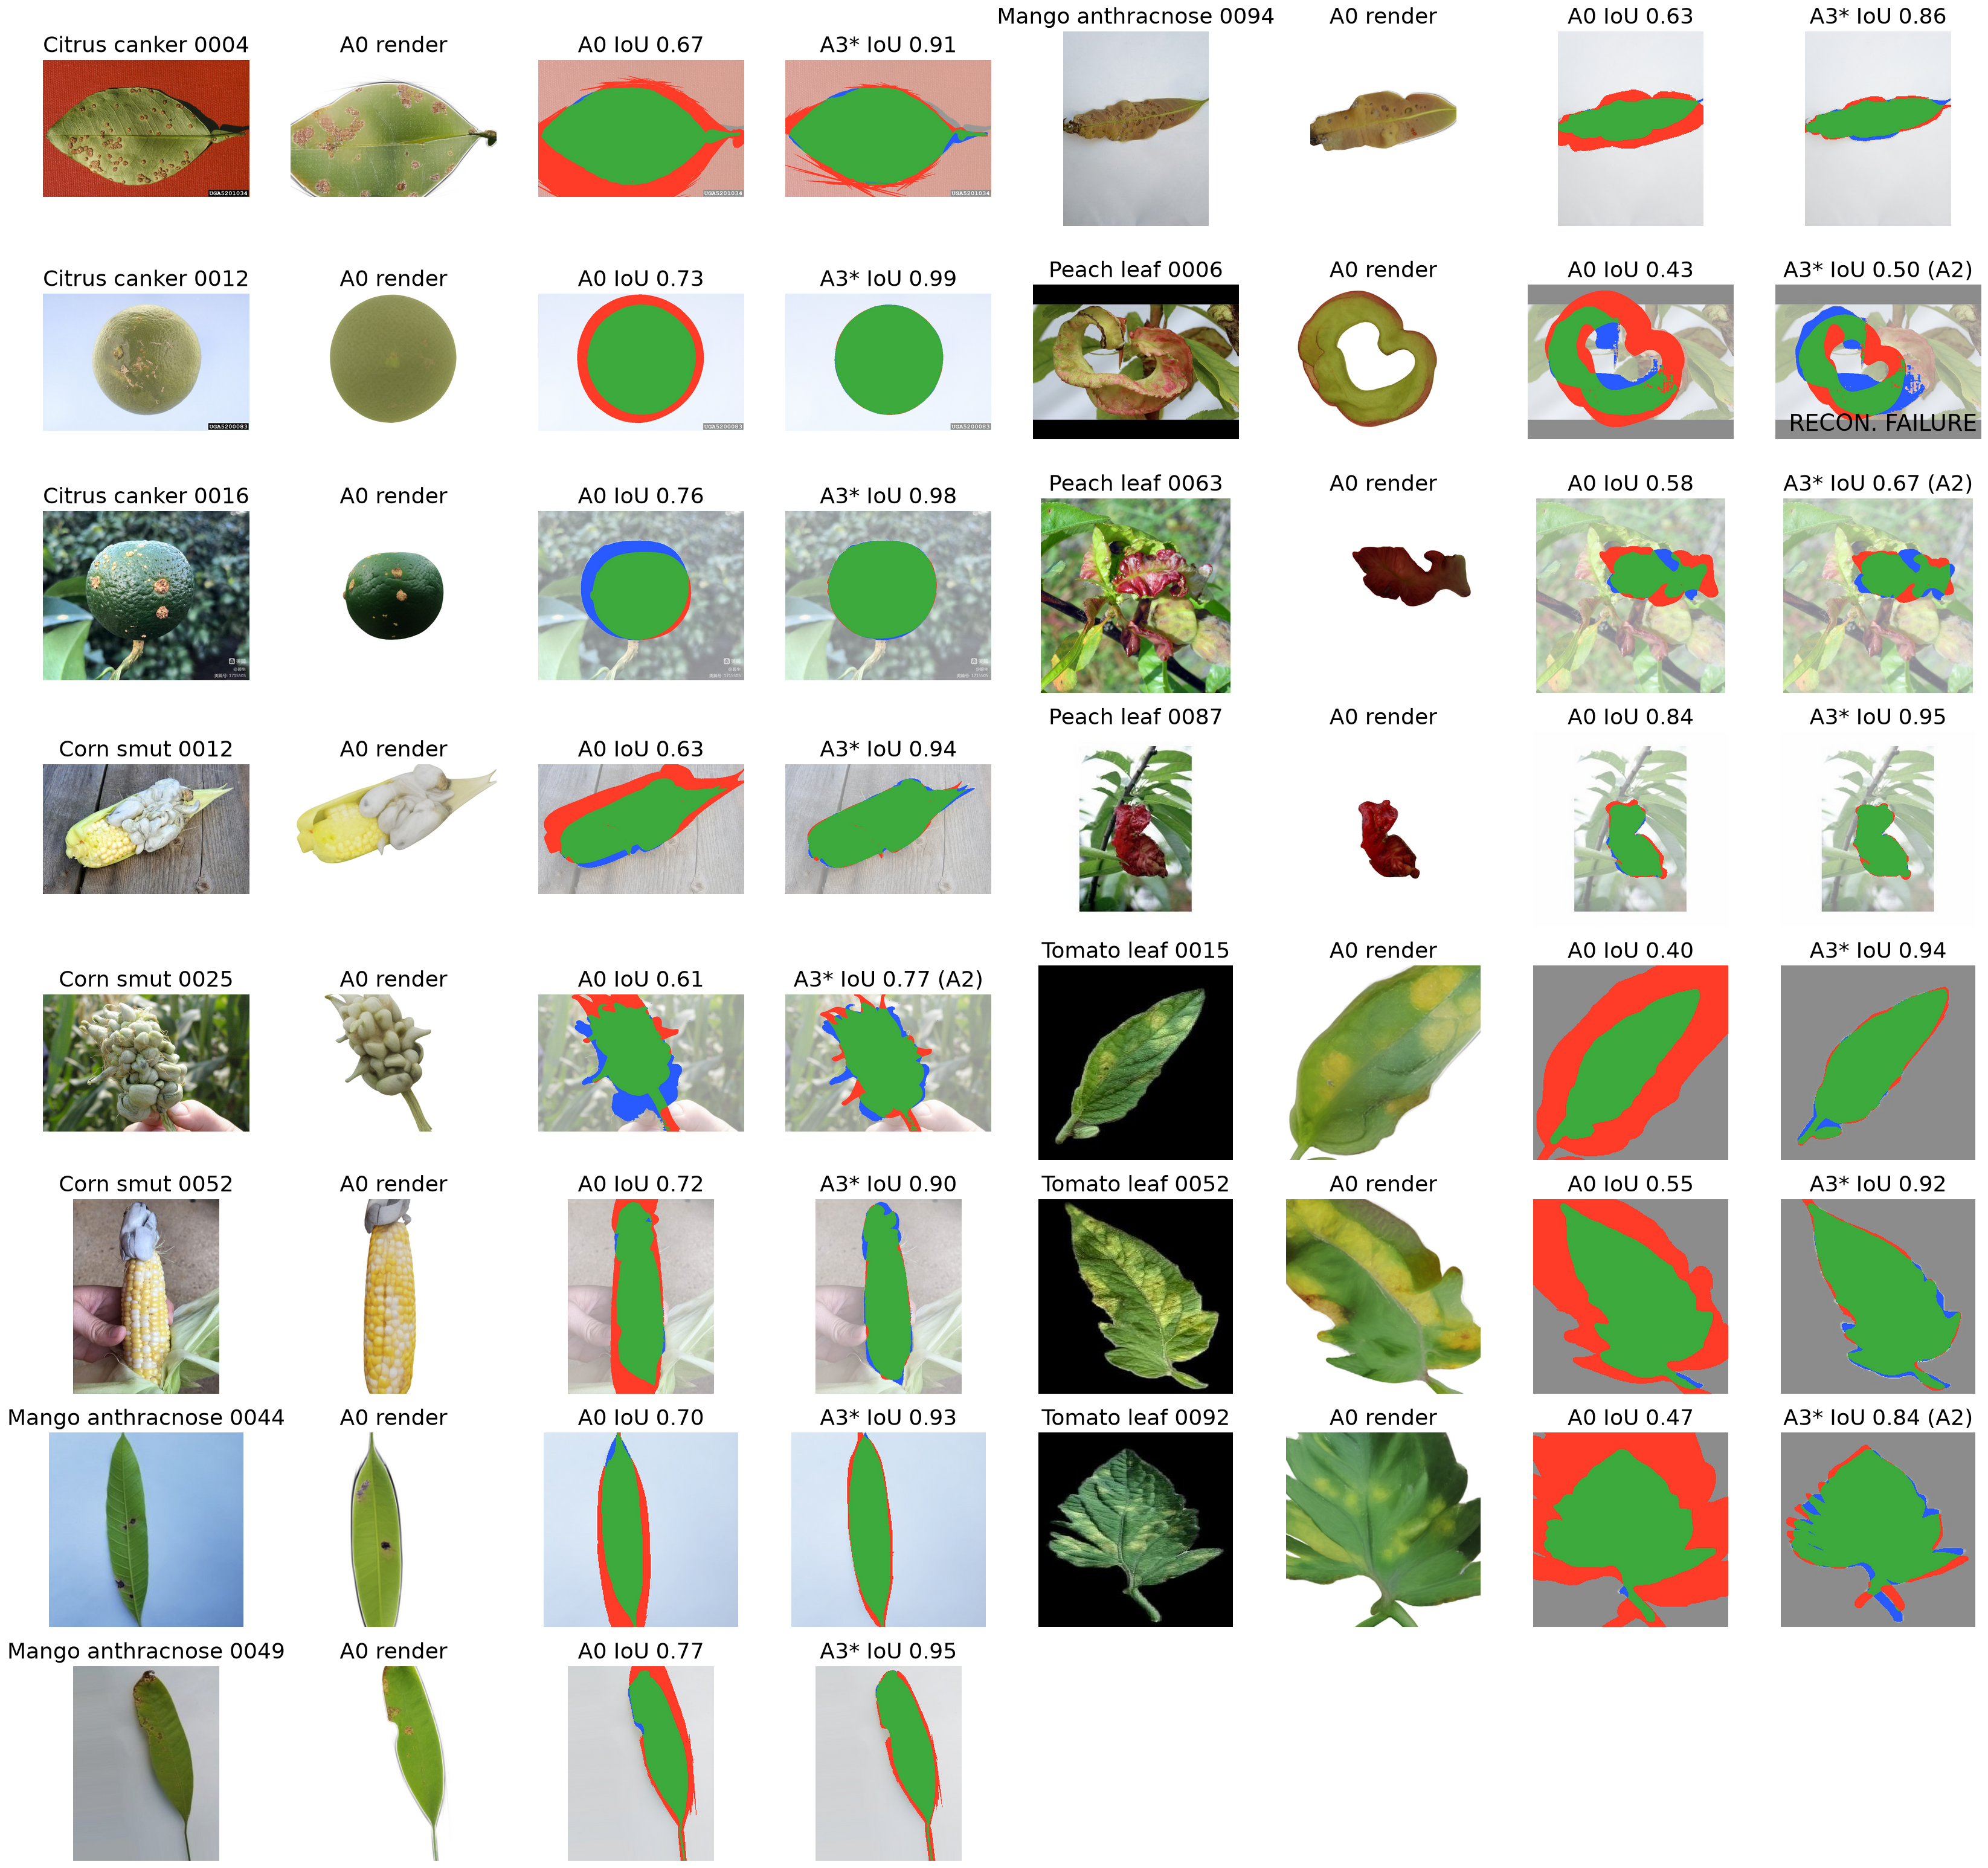
\includegraphics[width=\linewidth]{figs/fig2_alignment.png}\caption{Reconstruction debugging: A0 vs corrected pose A3*. Fitted, not verified.}\end{figure}

\subsection{What GaussianEditor changes}
\begin{figure}[H]\centering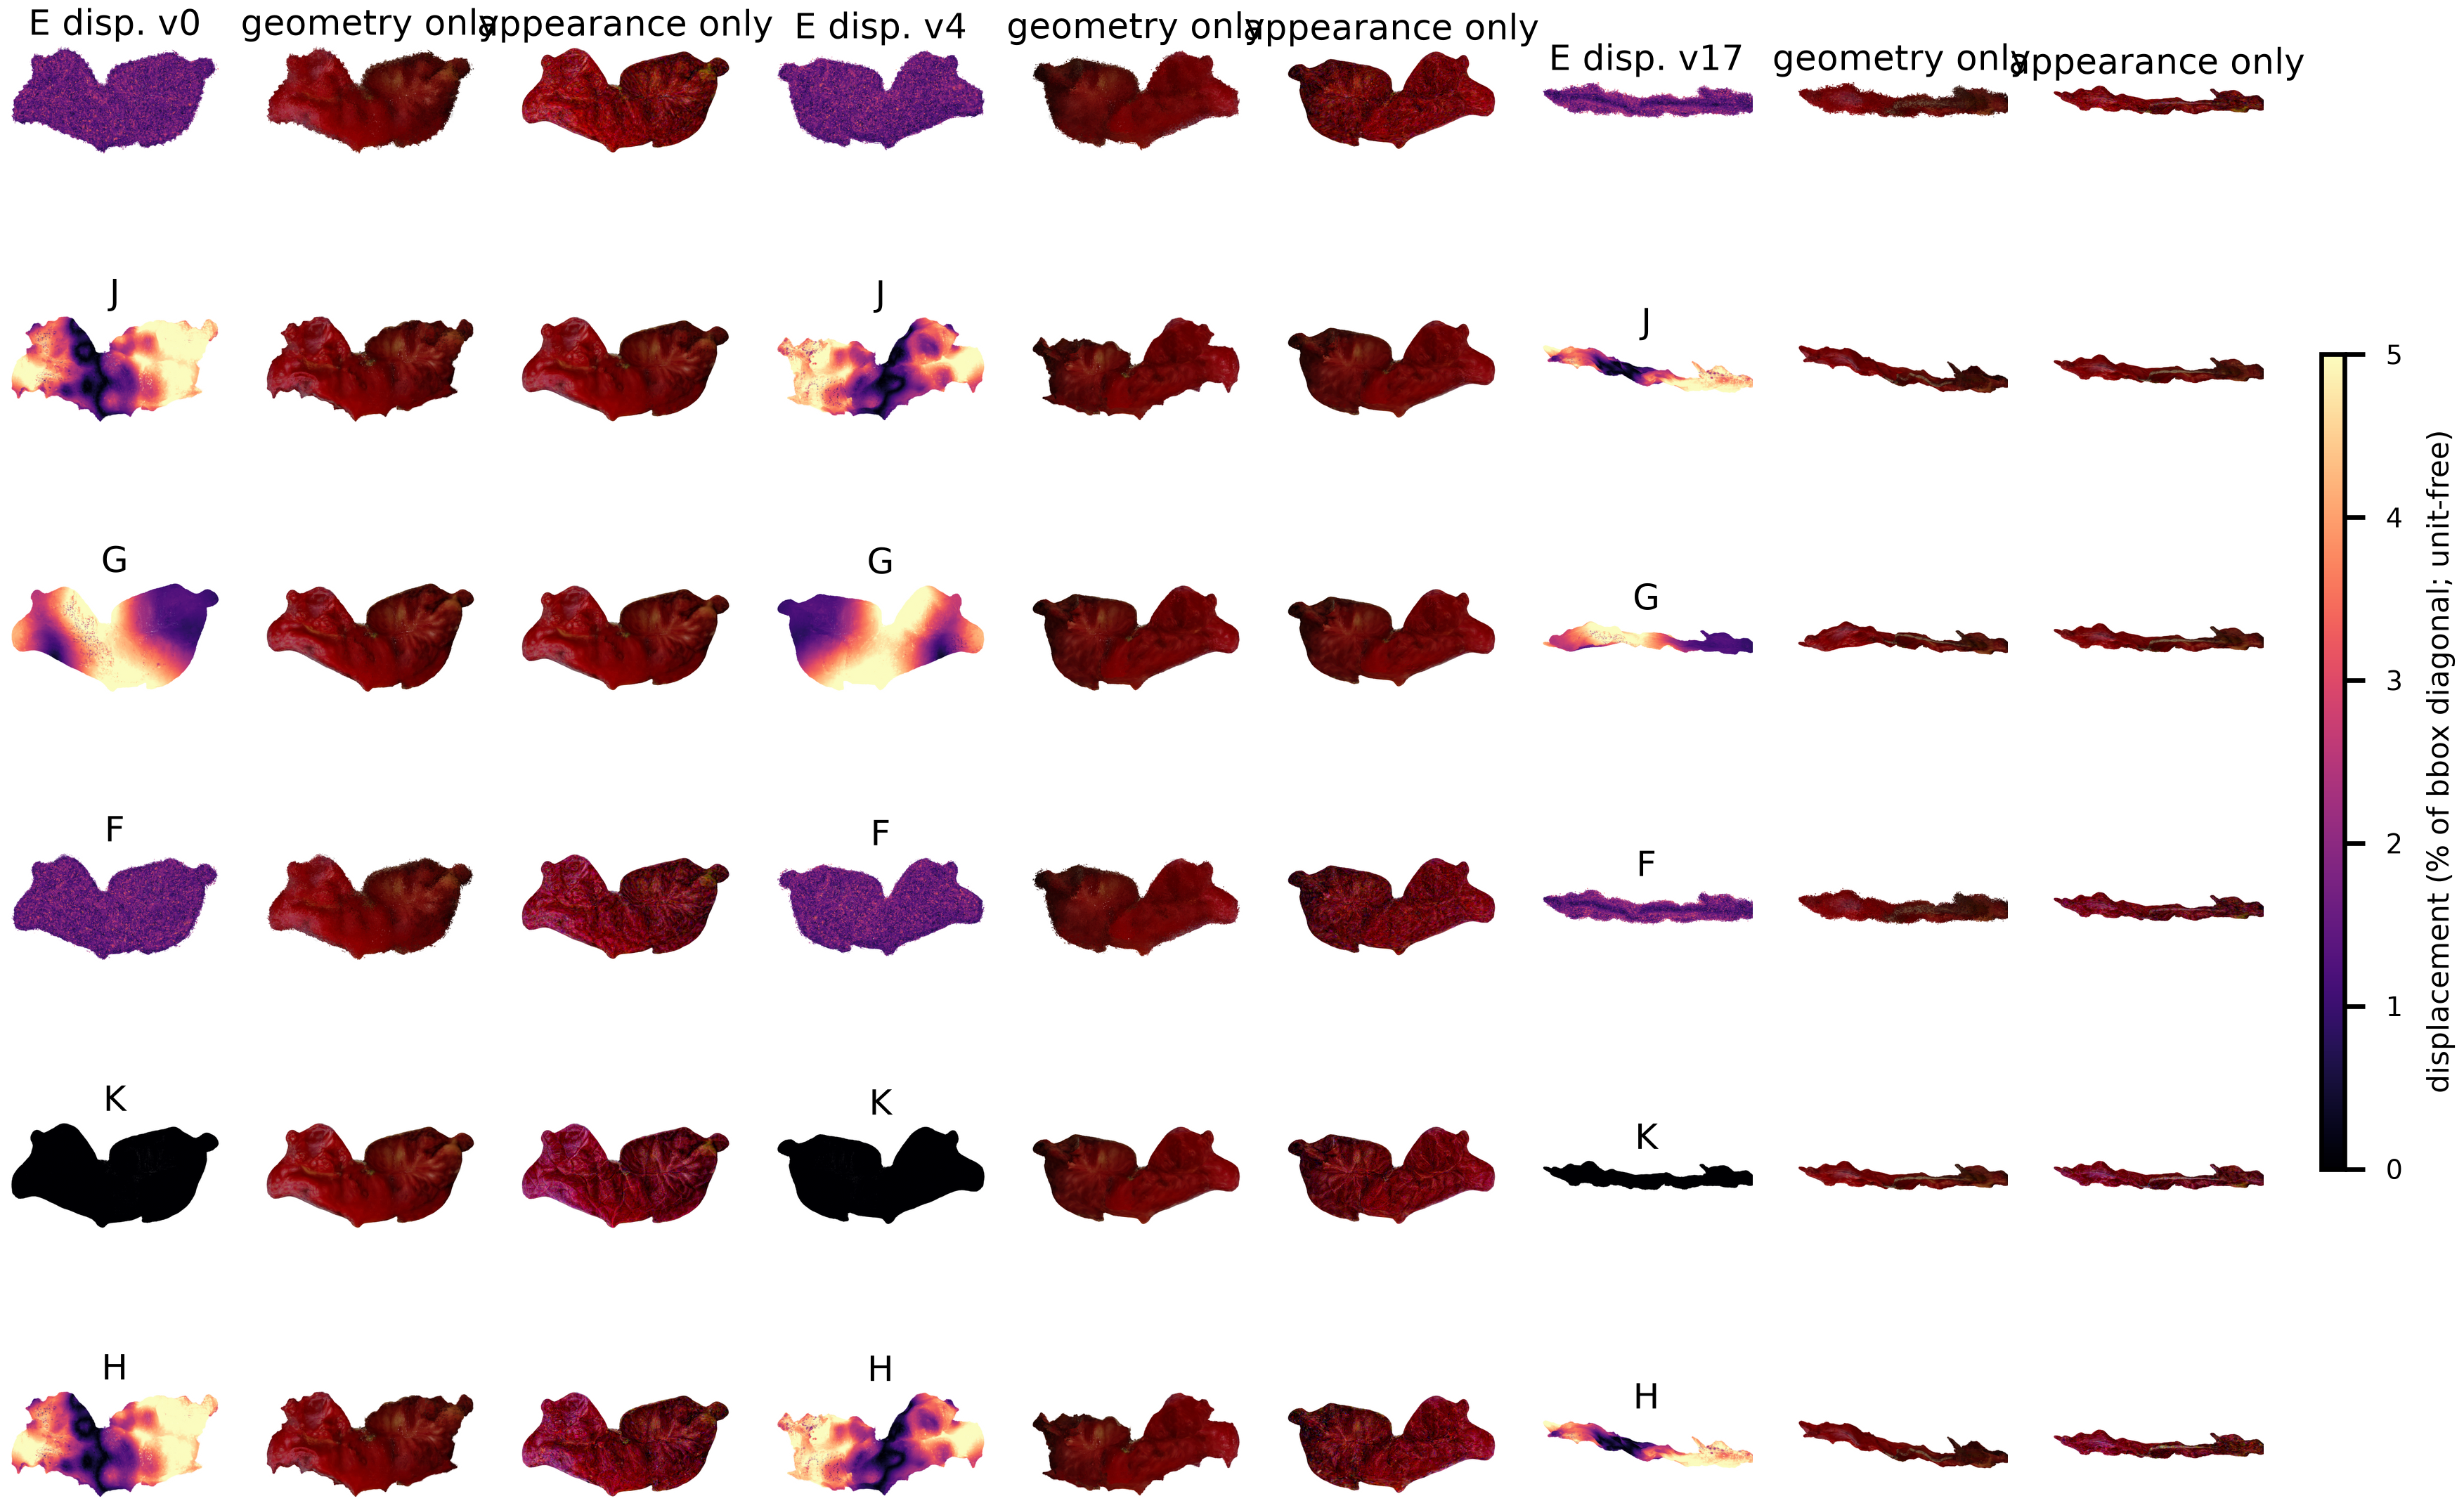
\includegraphics[width=\linewidth]{figs/fig5_displacement_Peach__Leaf_Curl__0087.png}\caption{Displacement heatmaps and geometry-only / appearance-only decomposition (Peach 0087).}\end{figure}

\subsection{Geometry-aware editing and knowledge ablation}
\begin{figure}[H]\centering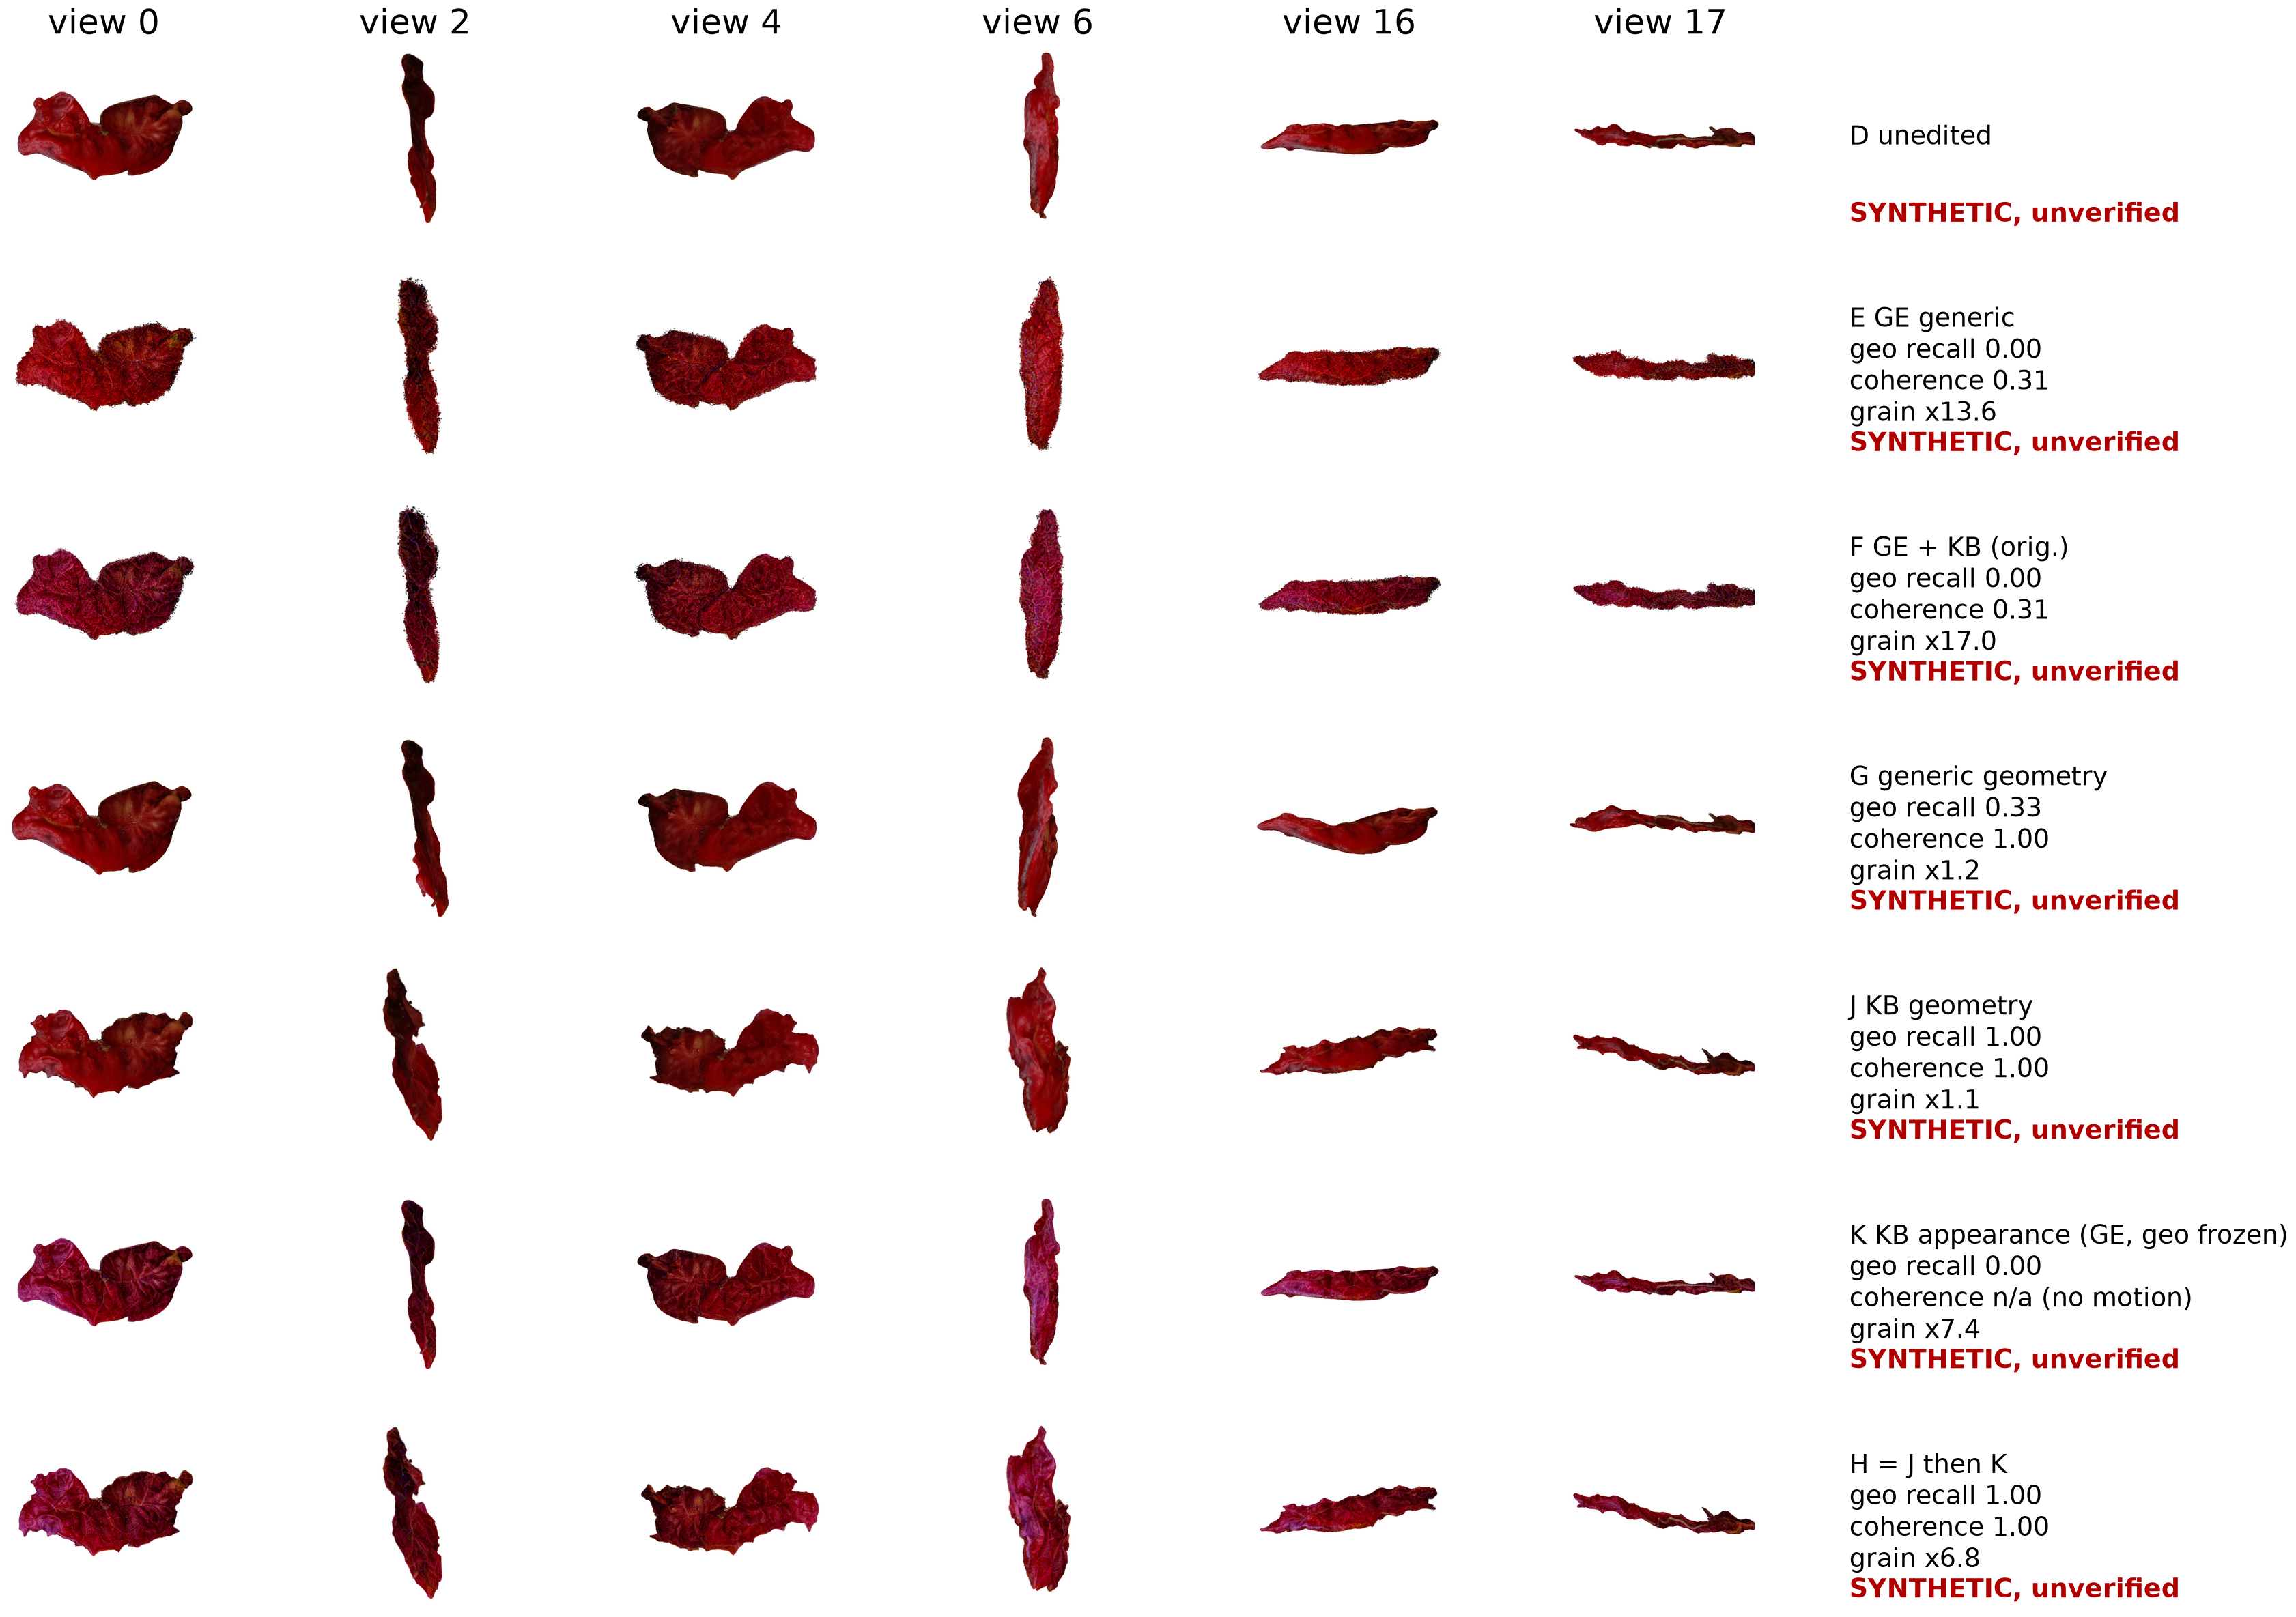
\includegraphics[width=\linewidth]{figs/fig3_editing_Peach__Leaf_Curl__0087.png}\caption{All 3D arms of Peach 0087 on fixed rig views (synthetic, unverified).}\end{figure}

\begin{figure}[H]\centering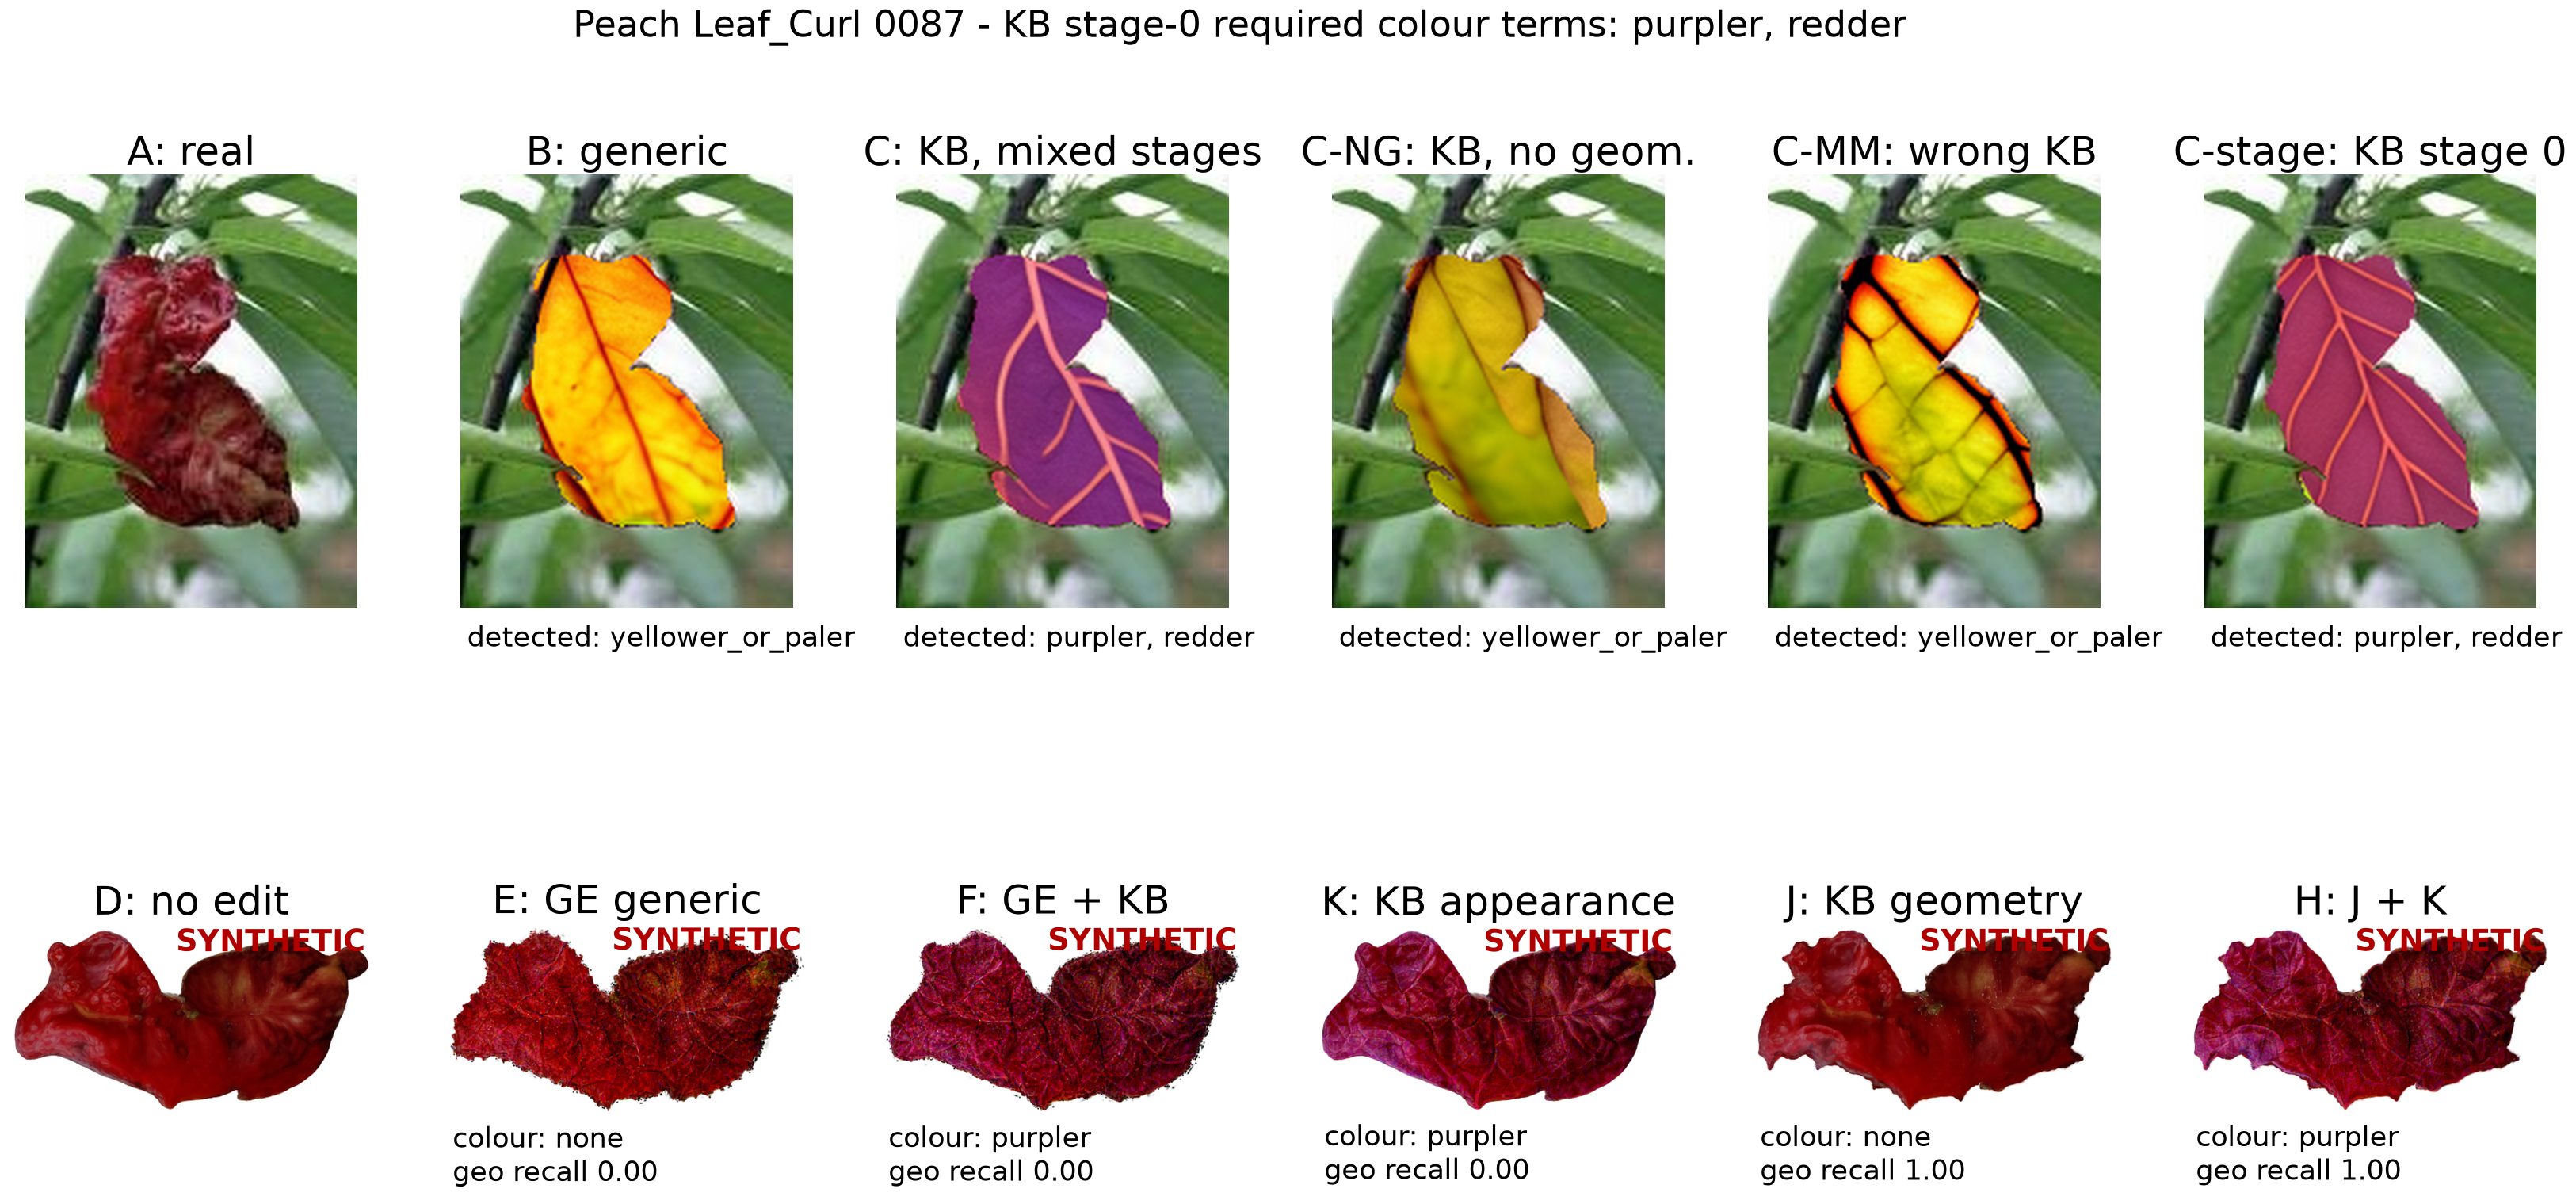
\includegraphics[width=\linewidth]{figs/fig4_kb_ablation_Peach__Leaf_Curl__0087.png}\caption{Knowledge ablation in 2D and 3D on Peach 0087.}\end{figure}

\begin{figure}[H]\centering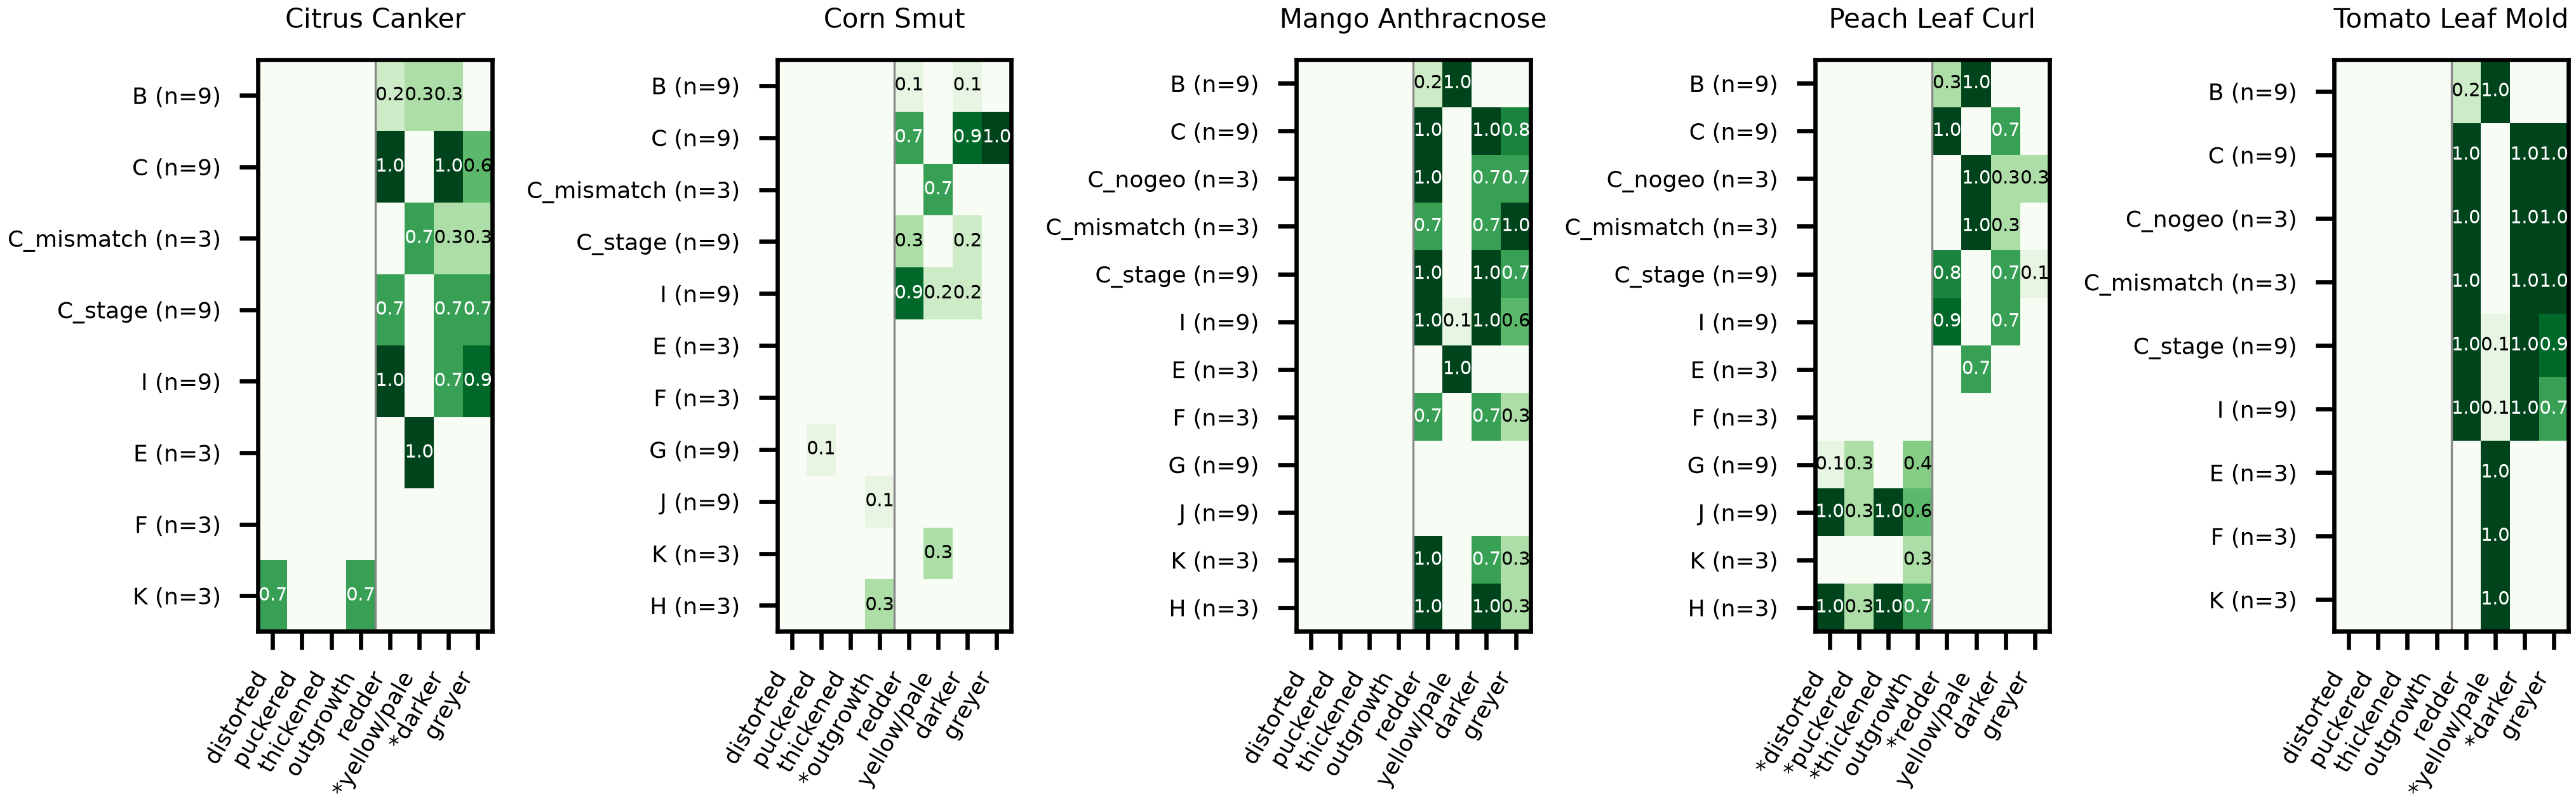
\includegraphics[width=\linewidth]{figs/fig6_attributes.png}\caption{Requested (KB) vs realised attributes per class.}\end{figure}

\begin{table}[H]\centering\scriptsize
\caption{Per-specimen metrics (seeds averaged). Recalls over specific detectors / scorable colour terms; -- = not applicable or not scorable.}
\resizebox{\linewidth}{!}{
\begin{tabular}{lrrrrrrrrrr}\toprule
Specimen & Arm & seeds & geo recall & app recall & unsupp. geo & coherence & sil.\ change & grain & fuzz & $\Delta$E \\ \midrule
Citrus Canker 0004 & D & 1 & -- & 0.00 & 0.00 & -- & 0.00 & 1.0 & 1.0 & 0.0 \\
Citrus Canker 0004 & E & 1 & -- & 0.50 & 0.00 & 0.31 & 0.17 & 2.9 & 1.6 & 22.0 \\
Citrus Canker 0004 & F & 1 & -- & 0.00 & 0.00 & 0.31 & 0.18 & 3.3 & 1.5 & 16.5 \\
Citrus Canker 0004 & K & 1 & -- & 0.00 & 0.00 & 0.00 & 0.00 & 2.8 & 1.0 & 9.4 \\
Citrus Canker 0012 & D & 1 & -- & 0.00 & 0.00 & -- & 0.00 & 1.0 & 1.0 & 0.0 \\
Citrus Canker 0012 & E & 1 & -- & -- & 0.00 & 0.32 & 0.06 & 70.8 & 2.2 & 21.2 \\
Citrus Canker 0012 & F & 1 & -- & -- & 0.00 & 0.32 & 0.06 & 78.4 & 2.3 & 18.4 \\
Citrus Canker 0012 & K & 1 & -- & -- & 1.00 & 0.96 & 0.00 & 27.4 & 1.0 & 11.7 \\
Citrus Canker 0016 & D & 1 & -- & 0.00 & 0.00 & -- & 0.00 & 1.0 & 1.0 & 0.0 \\
Citrus Canker 0016 & E & 1 & -- & -- & 0.00 & 0.31 & 0.06 & 12.9 & 2.3 & 17.4 \\
Citrus Canker 0016 & F & 1 & -- & -- & 0.00 & 0.32 & 0.07 & 15.2 & 2.3 & 15.7 \\
Citrus Canker 0016 & K & 1 & -- & -- & 1.00 & 0.97 & 0.00 & 6.9 & 1.0 & 9.5 \\
Corn Smut 0012 & D & 1 & 0.00 & 0.00 & 0.00 & -- & 0.00 & 1.0 & 1.0 & 0.0 \\
Corn Smut 0012 & E & 1 & 0.00 & -- & 0.00 & 0.31 & 0.09 & 25.8 & 2.1 & 13.9 \\
Corn Smut 0012 & F & 1 & 0.00 & -- & 0.00 & 0.31 & 0.09 & 30.2 & 2.0 & 16.2 \\
Corn Smut 0012 & G & 3 & 0.00 & -- & 0.00 & 0.99 & 0.10 & 1.1 & 1.3 & 5.9 \\
Corn Smut 0012 & J & 3 & 0.00 & -- & 0.00 & 0.93 & 0.14 & 1.5 & 1.4 & 4.0 \\
Corn Smut 0012 & K & 1 & 0.00 & -- & 0.00 & 0.12 & 0.00 & 10.1 & 1.0 & 10.1 \\
Corn Smut 0012 & H & 1 & 0.00 & -- & 0.00 & 0.93 & 0.15 & 12.4 & 1.5 & 11.8 \\
Corn Smut 0025 & D & 1 & 0.00 & 0.00 & 0.00 & -- & 0.00 & 1.0 & 1.0 & 0.0 \\
Corn Smut 0025 & E & 1 & 0.00 & -- & 0.00 & 0.31 & 0.10 & 11.0 & 1.8 & 15.1 \\
Corn Smut 0025 & F & 1 & 0.00 & -- & 0.00 & 0.31 & 0.11 & 13.1 & 1.9 & 16.8 \\
Corn Smut 0025 & G & 3 & 0.00 & -- & 0.33 & 1.00 & 0.13 & 1.1 & 1.3 & 7.5 \\
Corn Smut 0025 & J & 3 & 0.00 & -- & 0.00 & 0.92 & 0.13 & 1.4 & 1.6 & 4.9 \\
Corn Smut 0025 & K & 1 & 0.00 & -- & 0.00 & 0.00 & 0.00 & 3.6 & 1.0 & 11.2 \\
Corn Smut 0025 & H & 1 & 0.00 & -- & 0.00 & 0.94 & 0.12 & 4.6 & 1.6 & 12.7 \\
Corn Smut 0052 & D & 1 & 0.00 & 0.00 & 0.00 & -- & 0.00 & 1.0 & 1.0 & 0.0 \\
Corn Smut 0052 & E & 1 & 0.00 & -- & 0.00 & 0.31 & 0.11 & 9.6 & 1.8 & 16.7 \\
Corn Smut 0052 & F & 1 & 0.00 & -- & 0.00 & 0.32 & 0.10 & 13.0 & 1.8 & 18.8 \\
Corn Smut 0052 & G & 3 & 0.00 & -- & 0.00 & 0.95 & 0.12 & 1.1 & 1.2 & 11.6 \\
Corn Smut 0052 & J & 3 & 0.33 & -- & 0.00 & 0.83 & 0.14 & 1.2 & 1.3 & 8.7 \\
Corn Smut 0052 & K & 1 & 0.00 & -- & 0.00 & 0.59 & 0.00 & 5.1 & 1.0 & 11.7 \\
Corn Smut 0052 & H & 1 & 1.00 & -- & 0.00 & 0.83 & 0.14 & 5.9 & 1.3 & 16.4 \\
Mango Anthracnose 0044 & D & 1 & -- & 0.00 & 0.00 & -- & 0.00 & 1.0 & 1.0 & 0.0 \\
Mango Anthracnose 0044 & E & 1 & -- & -- & 0.00 & 0.32 & 0.09 & 6.3 & 1.8 & 20.2 \\
Mango Anthracnose 0044 & F & 1 & -- & -- & 0.00 & 0.32 & 0.09 & 7.6 & 1.6 & 14.9 \\
Mango Anthracnose 0044 & G & 3 & -- & -- & 0.00 & 0.85 & 0.04 & 0.8 & 1.2 & 2.5 \\
Mango Anthracnose 0044 & J & 3 & -- & -- & 0.00 & 0.60 & 0.04 & 0.8 & 1.3 & 2.6 \\
Mango Anthracnose 0044 & K & 1 & -- & -- & 0.00 & 0.00 & 0.00 & 6.1 & 1.0 & 12.1 \\
Mango Anthracnose 0044 & H & 1 & -- & -- & 0.00 & 0.60 & 0.04 & 5.2 & 1.3 & 13.2 \\
Mango Anthracnose 0049 & D & 1 & -- & 0.00 & 0.00 & -- & 0.00 & 1.0 & 1.0 & 0.0 \\
Mango Anthracnose 0049 & E & 1 & -- & -- & 0.00 & 0.31 & 0.20 & 10.4 & 2.0 & 17.4 \\
Mango Anthracnose 0049 & F & 1 & -- & -- & 0.00 & 0.31 & 0.20 & 11.7 & 1.9 & 19.6 \\
Mango Anthracnose 0049 & G & 3 & -- & -- & 0.00 & 0.95 & 0.04 & 1.0 & 1.1 & 2.8 \\
Mango Anthracnose 0049 & J & 3 & -- & -- & 0.00 & 0.63 & 0.03 & 0.9 & 1.1 & 2.2 \\
Mango Anthracnose 0049 & K & 1 & -- & -- & 0.00 & 0.00 & 0.00 & 7.8 & 1.0 & 16.1 \\
Mango Anthracnose 0049 & H & 1 & -- & -- & 0.00 & 0.63 & 0.04 & 7.4 & 1.1 & 16.4 \\
Mango Anthracnose 0094 & D & 1 & -- & 0.00 & 0.00 & -- & 0.00 & 1.0 & 1.0 & 0.0 \\
Mango Anthracnose 0094 & E & 1 & -- & -- & 0.00 & 0.31 & 0.14 & 4.7 & 1.4 & 24.6 \\
Mango Anthracnose 0094 & F & 1 & -- & -- & 0.00 & 0.32 & 0.14 & 5.9 & 1.3 & 17.9 \\
Mango Anthracnose 0094 & G & 3 & -- & -- & 0.00 & 0.48 & 0.03 & 1.0 & 1.0 & 2.5 \\
Mango Anthracnose 0094 & J & 3 & -- & -- & 0.00 & 0.45 & 0.02 & 1.0 & 1.1 & 1.7 \\
Mango Anthracnose 0094 & K & 1 & -- & -- & 0.00 & 0.43 & 0.00 & 4.0 & 1.0 & 13.8 \\
Mango Anthracnose 0094 & H & 1 & -- & -- & 0.00 & 0.45 & 0.02 & 3.8 & 1.1 & 14.1 \\
Peach Leaf\_Curl 0006 & D & 1 & 0.00 & 0.00 & 0.00 & -- & 0.00 & 1.0 & 1.0 & 0.0 \\
Peach Leaf\_Curl 0006 & E & 1 & 0.00 & 0.00 & 0.00 & 0.32 & 0.12 & 20.5 & 2.2 & 22.1 \\
Peach Leaf\_Curl 0006 & F & 1 & 0.00 & 0.00 & 0.00 & 0.32 & 0.12 & 24.2 & 2.2 & 21.6 \\
Peach Leaf\_Curl 0006 & G & 3 & 0.00 & 0.00 & 1.00 & 0.98 & 0.21 & 1.2 & 1.3 & 10.2 \\
Peach Leaf\_Curl 0006 & J & 3 & 0.67 & 0.00 & 0.33 & 0.98 & 0.23 & 1.7 & 2.9 & 11.0 \\
Peach Leaf\_Curl 0006 & K & 1 & 0.00 & 0.00 & 1.00 & 0.97 & 0.00 & 11.0 & 1.0 & 17.2 \\
Peach Leaf\_Curl 0006 & H & 1 & 0.67 & 0.00 & 0.33 & 0.98 & 0.23 & 9.7 & 2.9 & 21.4 \\
Peach Leaf\_Curl 0063 & D & 1 & 0.00 & 0.00 & 0.00 & -- & 0.00 & 1.0 & 1.0 & 0.0 \\
Peach Leaf\_Curl 0063 & E & 1 & 0.00 & 0.00 & 0.00 & 0.32 & 0.11 & 14.6 & 1.9 & 16.4 \\
Peach Leaf\_Curl 0063 & F & 1 & 0.00 & 1.00 & 0.00 & 0.32 & 0.11 & 19.0 & 1.9 & 19.9 \\
Peach Leaf\_Curl 0063 & G & 3 & 0.33 & 0.00 & 0.00 & 0.97 & 0.20 & 1.1 & 1.2 & 12.1 \\
Peach Leaf\_Curl 0063 & J & 3 & 0.78 & 0.00 & 0.22 & 0.96 & 0.22 & 1.9 & 2.4 & 12.7 \\
Peach Leaf\_Curl 0063 & K & 1 & 0.00 & 1.00 & 0.00 & 0.92 & 0.00 & 8.4 & 1.0 & 15.9 \\
Peach Leaf\_Curl 0063 & H & 1 & 0.67 & 1.00 & 0.33 & 0.96 & 0.23 & 8.1 & 2.5 & 21.0 \\
Peach Leaf\_Curl 0087 & D & 1 & 0.00 & 0.00 & 0.00 & -- & 0.00 & 1.0 & 1.0 & 0.0 \\
Peach Leaf\_Curl 0087 & E & 1 & 0.00 & 0.00 & 0.00 & 0.31 & 0.14 & 13.6 & 1.9 & 13.5 \\
Peach Leaf\_Curl 0087 & F & 1 & 0.00 & 1.00 & 0.00 & 0.31 & 0.14 & 17.0 & 1.9 & 16.2 \\
Peach Leaf\_Curl 0087 & G & 3 & 0.11 & 0.00 & 0.17 & 1.00 & 0.23 & 1.1 & 1.1 & 9.0 \\
Peach Leaf\_Curl 0087 & J & 3 & 0.89 & 0.00 & 0.00 & 1.00 & 0.26 & 1.1 & 1.4 & 9.6 \\
Peach Leaf\_Curl 0087 & K & 1 & 0.00 & 1.00 & 0.00 & 0.00 & 0.00 & 7.4 & 1.0 & 12.3 \\
Peach Leaf\_Curl 0087 & H & 1 & 1.00 & 1.00 & 0.00 & 1.00 & 0.28 & 6.8 & 1.4 & 15.9 \\
Tomato Leaf\_Mold 0015 & D & 1 & -- & 0.00 & 0.00 & -- & 0.00 & 1.0 & 1.0 & 0.0 \\
Tomato Leaf\_Mold 0015 & E & 1 & -- & 0.50 & 0.00 & 0.31 & 0.18 & 17.5 & 1.8 & 22.1 \\
Tomato Leaf\_Mold 0015 & F & 1 & -- & 0.50 & 0.00 & 0.31 & 0.17 & 19.7 & 1.9 & 19.1 \\
Tomato Leaf\_Mold 0015 & K & 1 & -- & 0.50 & 0.00 & 0.31 & 0.00 & 11.3 & 1.0 & 15.4 \\
Tomato Leaf\_Mold 0052 & D & 1 & -- & 0.00 & 0.00 & -- & 0.00 & 1.0 & 1.0 & 0.0 \\
Tomato Leaf\_Mold 0052 & E & 1 & -- & 0.50 & 0.00 & 0.30 & 0.18 & 16.5 & 1.8 & 22.9 \\
Tomato Leaf\_Mold 0052 & F & 1 & -- & 0.50 & 0.00 & 0.31 & 0.17 & 18.4 & 1.8 & 19.3 \\
Tomato Leaf\_Mold 0052 & K & 1 & -- & 0.50 & 0.00 & 0.00 & 0.00 & 10.4 & 1.0 & 14.5 \\
Tomato Leaf\_Mold 0092 & D & 1 & -- & 0.00 & 0.00 & -- & 0.00 & 1.0 & 1.0 & 0.0 \\
Tomato Leaf\_Mold 0092 & E & 1 & -- & 0.50 & 0.00 & 0.31 & 0.14 & 17.6 & 1.9 & 21.6 \\
Tomato Leaf\_Mold 0092 & F & 1 & -- & 0.50 & 0.00 & 0.31 & 0.14 & 19.2 & 1.9 & 18.8 \\
Tomato Leaf\_Mold 0092 & K & 1 & -- & 0.50 & 0.00 & 0.42 & 0.00 & 8.5 & 1.0 & 15.2 \\
\bottomrule\end{tabular}}\end{table}


\begin{table}[H]\centering\scriptsize
\caption{Specimen-level paired comparisons (seeds averaged within specimen). Cluster bootstrap over disease classes; $^\ast$ fewer than 3 classes, so the cluster CI is degenerate or unreliable (specimen-bootstrap CI shown as sensitivity). With n $\le$ 9 the Wilcoxon test cannot reach p $<$ 0.05 for n $<$ 6; CIs and sign counts are the primary summary.}
\resizebox{\linewidth}{!}{
\begin{tabular}{lrrrrrrrrr}\toprule
Comparison & Metric & n (classes) & mean a & mean b & diff [cluster CI] & specimen CI & a$>$b / a$<$b & Wilcoxon p & Holm p \\ \midrule
J vs G & geometry\_recall & 6 (2) & 0.44 & 0.07 & +0.37 [+0.11, +0.63]$^\ast$ & [+0.13, +0.61] & 4/0 & 0.125 & 0.875 \\
J vs G & unsupported\_rate & 9 (3) & 0.06 & 0.17 & -0.10 [-0.20, +0.00] & [-0.28, +0.03] & 1/3 & 0.375 & 1.000 \\
J vs E & coherence & 9 (3) & 0.81 & 0.31 & +0.50 [+0.25, +0.66] & [+0.37, +0.61] & 9/0 & 0.004 & 0.043 \\
J vs E & grain\_ratio & 9 (3) & 1.28 & 12.94 & -11.66 [-14.68, -6.20] & [-15.89, -7.94] & 0/9 & 0.004 & 0.043 \\
K vs E & appearance\_recall & 7 (3) & 0.50 & 0.29 & +0.21 [-0.50, +0.67] & [-0.14, +0.57] & 2/1 & 0.500 & 1.000 \\
K vs E & grain\_ratio & 15 (5) & 8.71 & 16.98 & -8.27 [-12.81, -4.00] & [-14.15, -4.24] & 0/15 & 0.000 & 0.001 \\
K vs E & fuzz\_ratio & 15 (5) & 1.00 & 1.90 & -0.90 [-1.00, -0.79] & [-1.01, -0.78] & 0/15 & 0.000 & 0.001 \\
H vs F & geometry\_recall & 6 (2) & 0.56 & 0.00 & +0.56 [+0.33, +0.78]$^\ast$ & [+0.22, +0.89] & 4/0 & 0.125 & 0.875 \\
H vs F & appearance\_recall & 3 (1) & 0.67 & 0.67 & +0.00 [+0.00, +0.00]$^\ast$ & [+0.00, +0.00] & 0/0 & -- & -- \\
H vs F & grain\_ratio & 9 (3) & 7.09 & 15.73 & -8.64 [-11.86, -2.93] & [-11.96, -5.45] & 0/9 & 0.004 & 0.043 \\
F vs E & appearance\_recall & 7 (3) & 0.50 & 0.29 & +0.21 [-0.50, +0.67] & [-0.14, +0.57] & 2/1 & 0.500 & 1.000 \\
H vs G & appearance\_recall & 3 (1) & 0.67 & 0.00 & +0.67 [+0.67, +0.67]$^\ast$ & [+0.00, +1.00] & 2/0 & 0.500 & 1.000 \\
H vs G & geometry\_recall & 6 (2) & 0.56 & 0.07 & +0.48 [+0.33, +0.63]$^\ast$ & [+0.17, +0.80] & 4/0 & 0.125 & 0.875 \\
F vs E & coherence & 15 (5) & 0.31 & 0.31 & +0.00 [+0.00, +0.00] & [+0.00, +0.00] & 11/4 & 0.030 & 0.241 \\
K vs E & appearance\_recall\_v1 & 3 (1) & 0.00 & 0.00 & +0.00 [+0.00, +0.00]$^\ast$ & [+0.00, +0.00] & 0/0 & -- & -- \\
F vs E & appearance\_recall\_v1 & 3 (1) & 0.00 & 0.00 & +0.00 [+0.00, +0.00]$^\ast$ & [+0.00, +0.00] & 0/0 & -- & -- \\
\bottomrule\end{tabular}}\end{table}


\begin{table}[H]\centering\scriptsize
\caption{Geometry $\times$ KB-conditioning ablation (mean over specimens with all four arms).}
{
\begin{tabular}{lr}\toprule
Cell & total KB recall \\ \midrule
D (no geo, no KB) & 0.00 \\
K (no geo, KB) & 0.17 \\
G (geo, no KB) & 0.04 \\
H (geo, KB) & 0.53 \\
interaction (H$-$G)$-$(K$-$D) & 0.32 \\
specimens with all four cells & 6 \\
\bottomrule\end{tabular}}\end{table}


\subsection{2D baselines}
\begin{table}[H]\centering\scriptsize\caption{2D arms vs the real photo (specimen-averaged). Outside-mask change = changed area outside the organ mask $\div$ organ area (shape-change capacity).}\begin{tabular}{lrrrrr}\toprule Arm & n & $\Delta$E in organ & outside change & KB colour recall & unsupported colours\\\midrule
B & 15 & 32.8 & 0.00 & 0.38 & 0.48\\
C & 15 & 47.1 & 0.00 & 0.71 & 0.77\\
C\_nogeo & 9 & 42.5 & 0.00 & 0.25 & 0.91\\
C\_mismatch & 15 & 37.4 & 0.00 & 0.29 & 0.85\\
C\_stage & 15 & 36.8 & 0.00 & 0.69 & 0.58\\
I & 15 & 43.3 & 0.83 & 0.74 & 0.74\\
\bottomrule\end{tabular}\end{table}
\subsection{Cross-view consistency}
\begin{table}[H]\centering\scriptsize
\caption{Correspondence-based cross-view consistency: median CIELAB $\Delta$E of the same surface point between adjacent ring views (lower = more consistent). Internal consistency only.}
\resizebox{\linewidth}{!}{
\begin{tabular}{lrrrrrrrrr}\toprule
Specimen & D floor & Bmv & Cmv & E & F & K & J & G & H \\ \midrule
Citrus Canker 0004 & 4.0 & 11.9 & 18.6 & 9.6 & 10.2 & 10.5 & -- & -- & -- \\
Citrus Canker 0012 & 1.3 & 5.5 & 7.9 & 9.4 & 10.9 & 12.0 & -- & -- & -- \\
Citrus Canker 0016 & 2.0 & 12.7 & 15.3 & 9.0 & 9.1 & 10.4 & -- & -- & -- \\
Corn Smut 0012 & 1.7 & 11.2 & 11.6 & 8.6 & 9.8 & 8.3 & 1.8 & 1.8 & 8.6 \\
Corn Smut 0025 & 2.3 & 14.0 & 8.0 & 10.0 & 10.8 & 8.1 & 2.3 & 2.4 & 8.7 \\
Corn Smut 0052 & 3.5 & 17.7 & 8.7 & 9.3 & 10.4 & 9.1 & 3.7 & 3.8 & 9.7 \\
Mango Anthracnose 0044 & 0.7 & 8.0 & 36.2 & 5.1 & 7.3 & 7.5 & 0.8 & 0.8 & 7.6 \\
Mango Anthracnose 0049 & 1.0 & 19.6 & 29.5 & 8.5 & 11.2 & 9.9 & 1.0 & 1.1 & 9.8 \\
Mango Anthracnose 0094 & 1.6 & 15.6 & 36.0 & 10.4 & 10.8 & 8.7 & 1.6 & 1.7 & 9.1 \\
Peach Leaf\_Curl 0006 & 2.4 & 28.6 & 27.6 & 10.6 & 11.8 & 10.0 & 2.9 & 2.3 & 11.2 \\
Peach Leaf\_Curl 0063 & 3.6 & 21.2 & 29.9 & 7.9 & 9.9 & 9.7 & 3.4 & 3.7 & 11.2 \\
Peach Leaf\_Curl 0087 & 2.1 & 21.7 & 32.9 & 7.4 & 9.6 & 9.0 & 2.0 & 2.0 & 9.5 \\
Tomato Leaf\_Mold 0015 & 2.0 & 16.8 & 18.3 & 10.1 & 10.8 & 8.6 & -- & -- & -- \\
Tomato Leaf\_Mold 0052 & 2.2 & 23.8 & 19.3 & 10.6 & 11.0 & 9.2 & -- & -- & -- \\
Tomato Leaf\_Mold 0092 & 1.7 & 19.5 & 24.0 & 8.7 & 9.7 & 7.8 & -- & -- & -- \\
\bottomrule\end{tabular}}\end{table}


\begin{figure}[H]\centering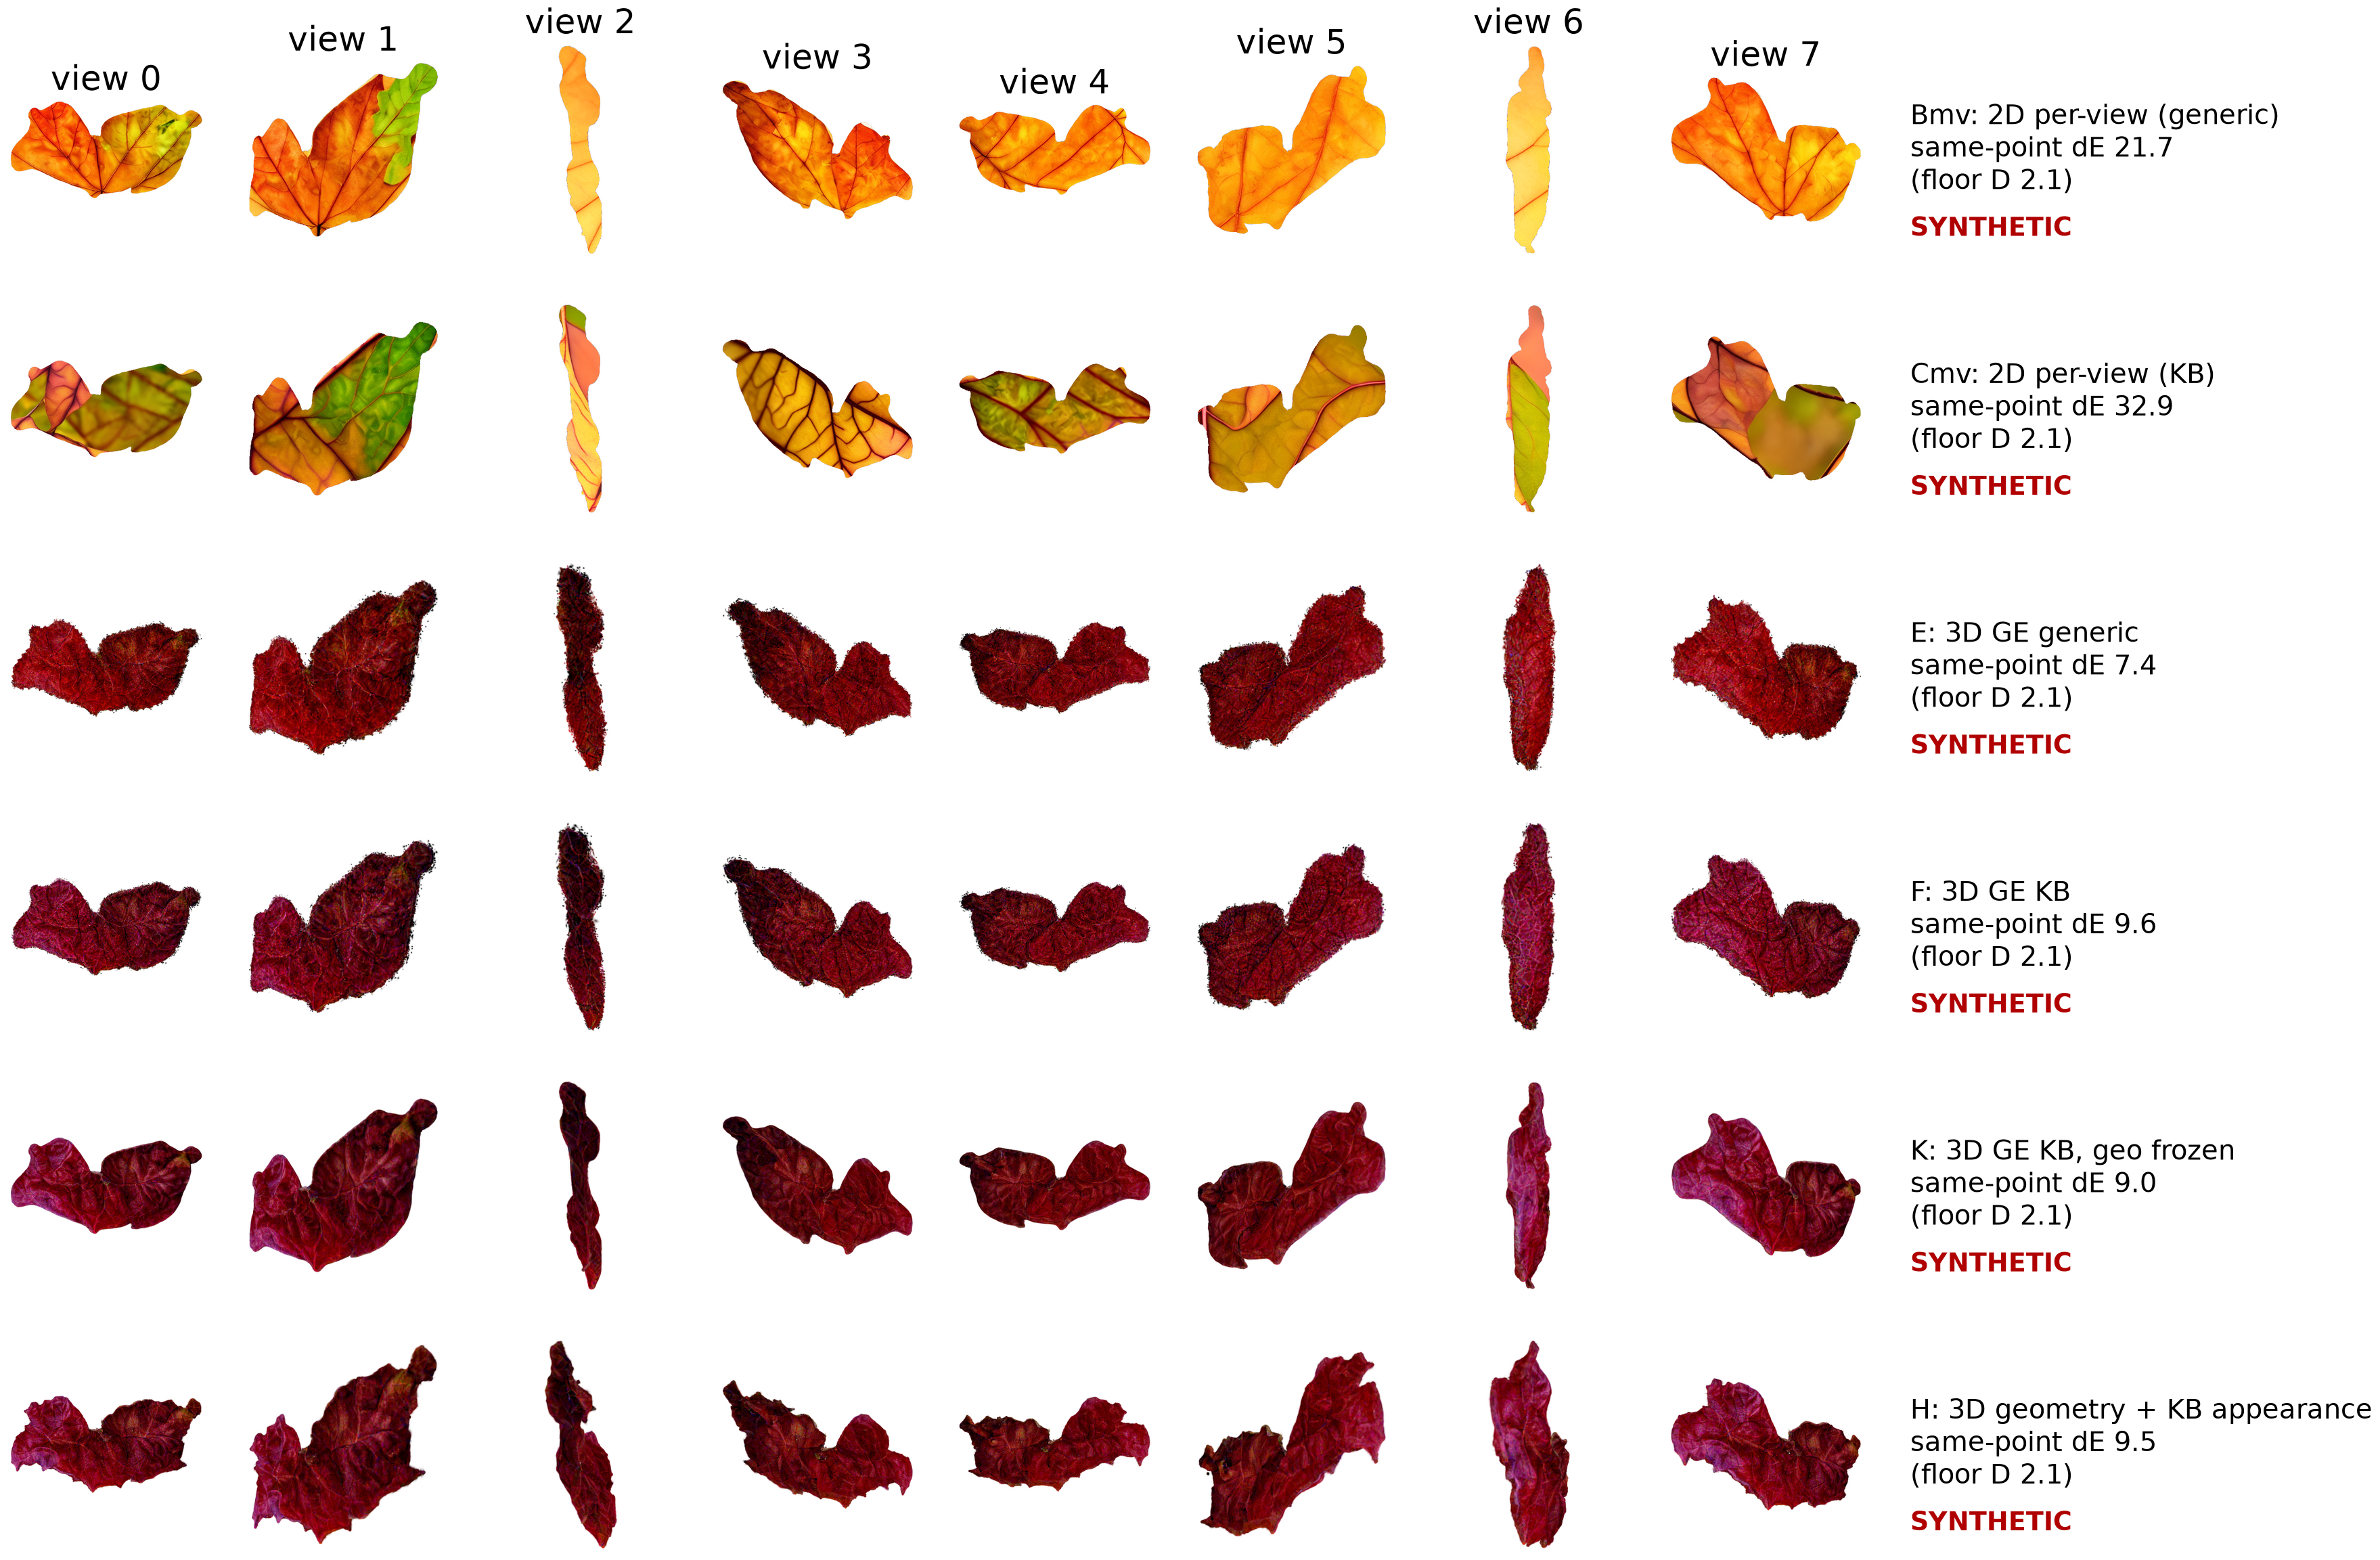
\includegraphics[width=\linewidth]{figs/fig7_crossview_Peach__Leaf_Curl__0087.png}\caption{Per-view 2D edits vs one 3D asset (Peach 0087).}\end{figure}

\subsection{Quality control and failures}
\begin{table}[H]\centering\scriptsize
\caption{Automated technical QC: number of flagged assets per arm (seed-level). Technical QC is not biological validation.}
\resizebox{\linewidth}{!}{
\begin{tabular}{lrrrrrr}\toprule
Flag & E & F & G & H & J & K \\ \midrule
exploding\_deformation & 0/15 & 0/15 & 3/27 & 1/15 & 3/27 & 3/15 \\
fuzzy\_edges & 13/15 & 12/15 & 0/27 & 2/15 & 6/27 & 0/15 \\
ge\_unverified & 3/15 & 0/15 & 0/27 & 0/15 & 0/27 & 0/15 \\
grainy\_texture & 15/15 & 15/15 & 0/27 & 9/15 & 6/27 & 15/15 \\
missing\_output & 0/15 & 0/15 & 0/27 & 6/15 & 0/27 & 0/15 \\
specimen\_reconstruction\_failure & 1/15 & 1/15 & 3/27 & 1/15 & 3/27 & 1/15 \\
unsupported\_appearance & 7/15 & 2/15 & 0/27 & 3/15 & 0/27 & 4/15 \\
unsupported\_geometry & 0/15 & 0/15 & 5/27 & 2/15 & 5/27 & 3/15 \\
\bottomrule\end{tabular}}\end{table}


\begin{figure}[H]\centering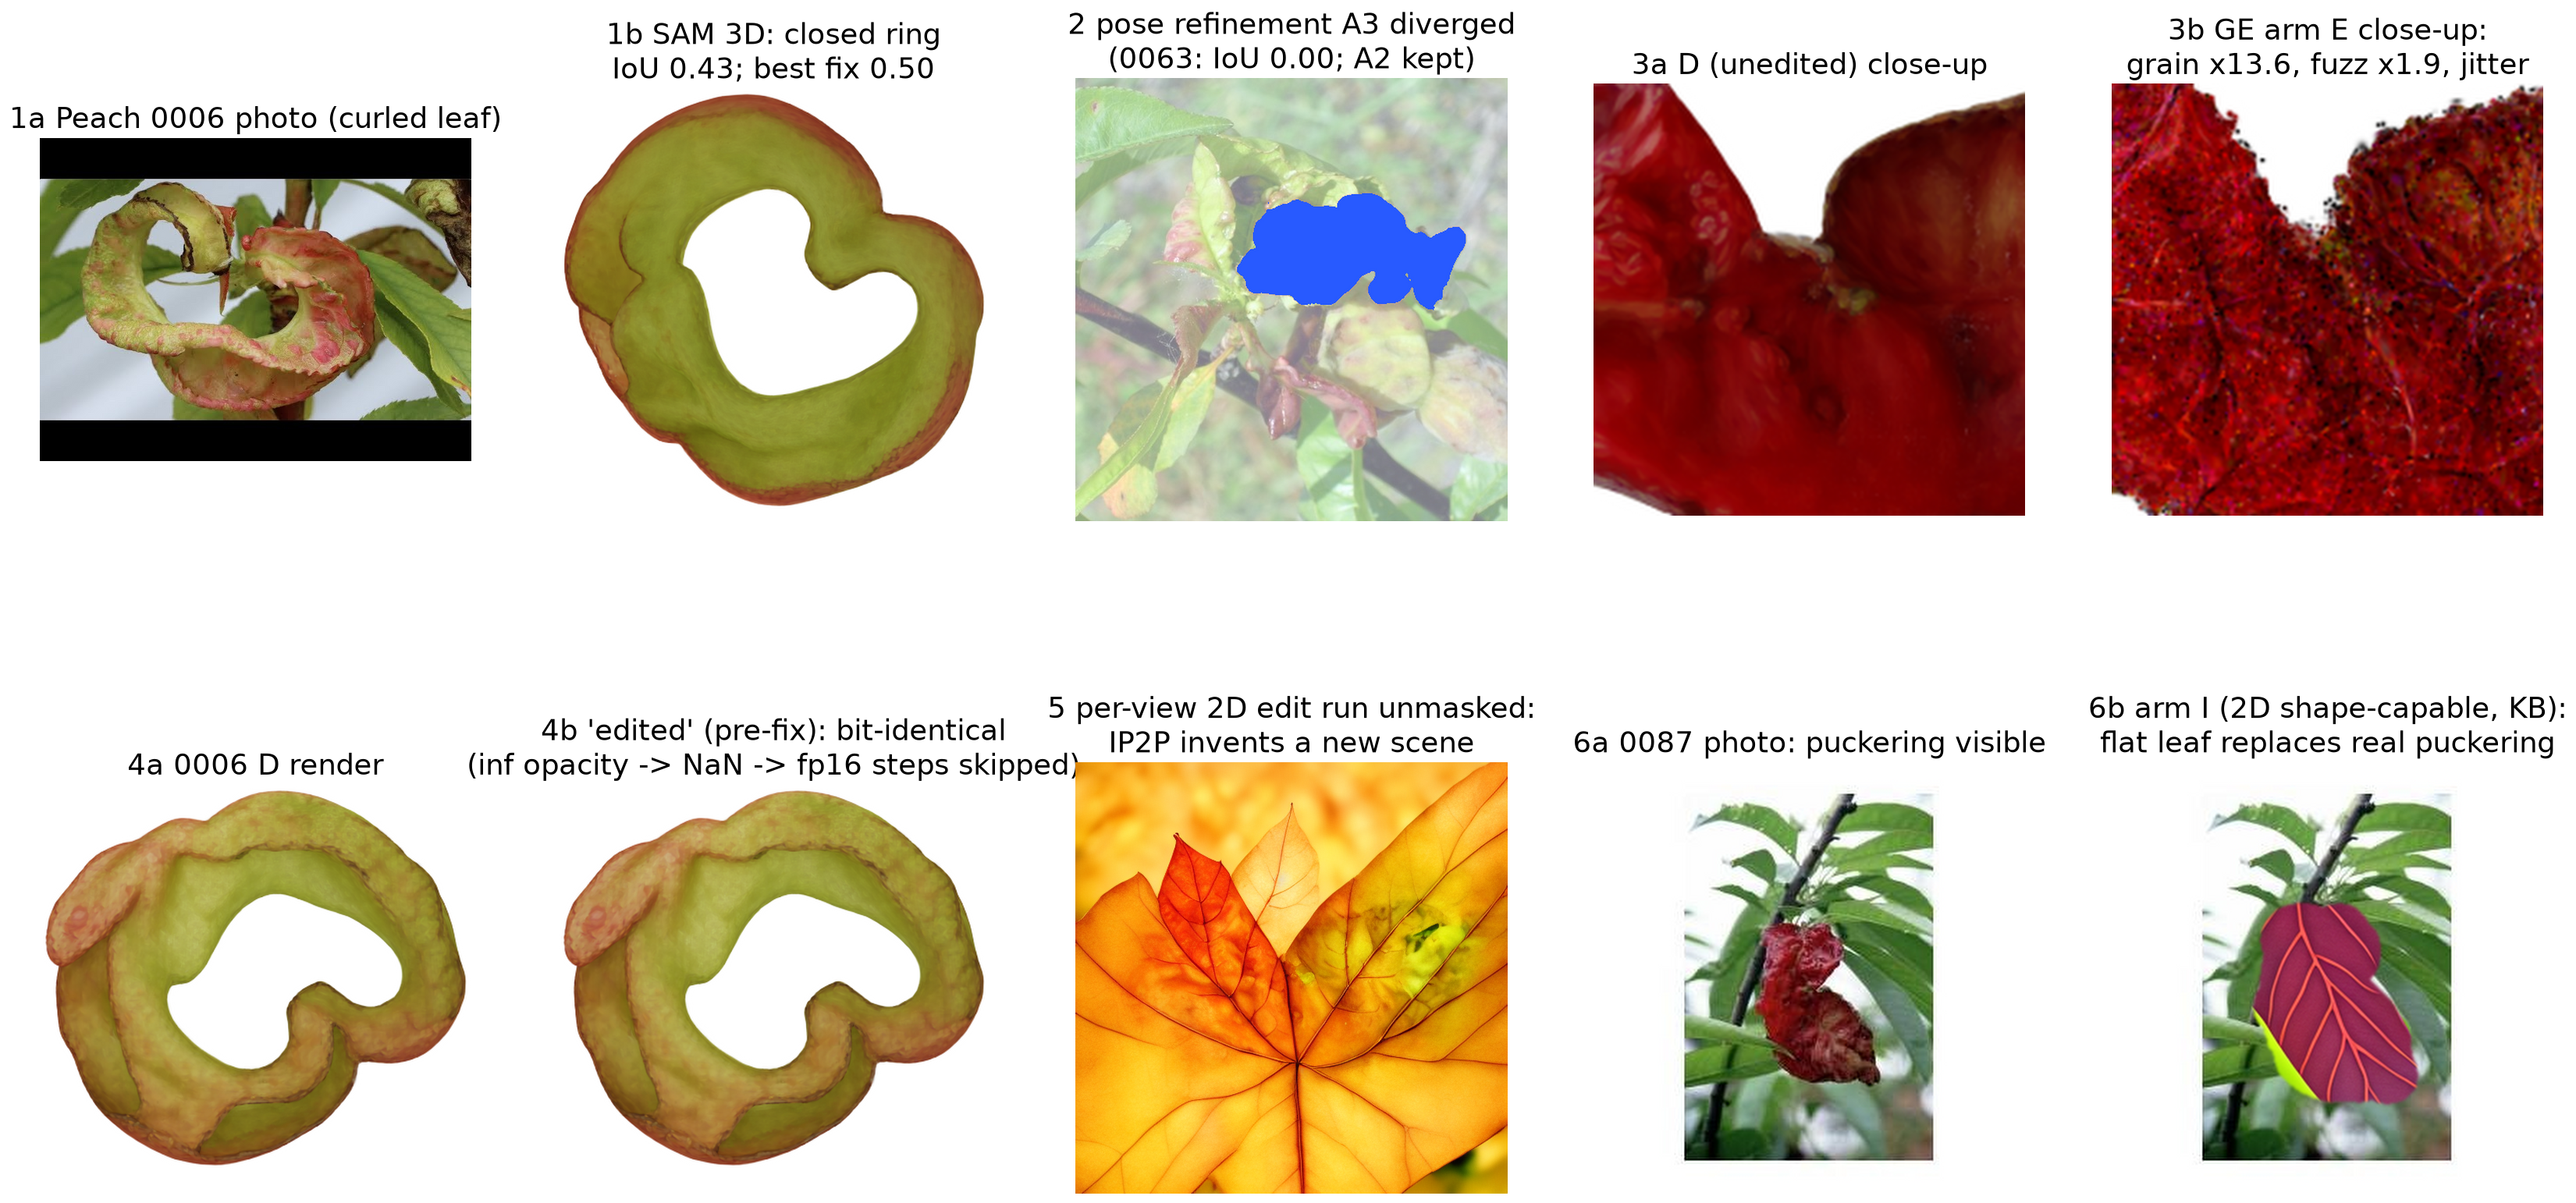
\includegraphics[width=\linewidth]{figs/fig9_failures.png}\caption{Failure taxonomy (real runs).}\end{figure}

\subsection{What 3D adds, and what it does not}
\begin{figure}[H]\centering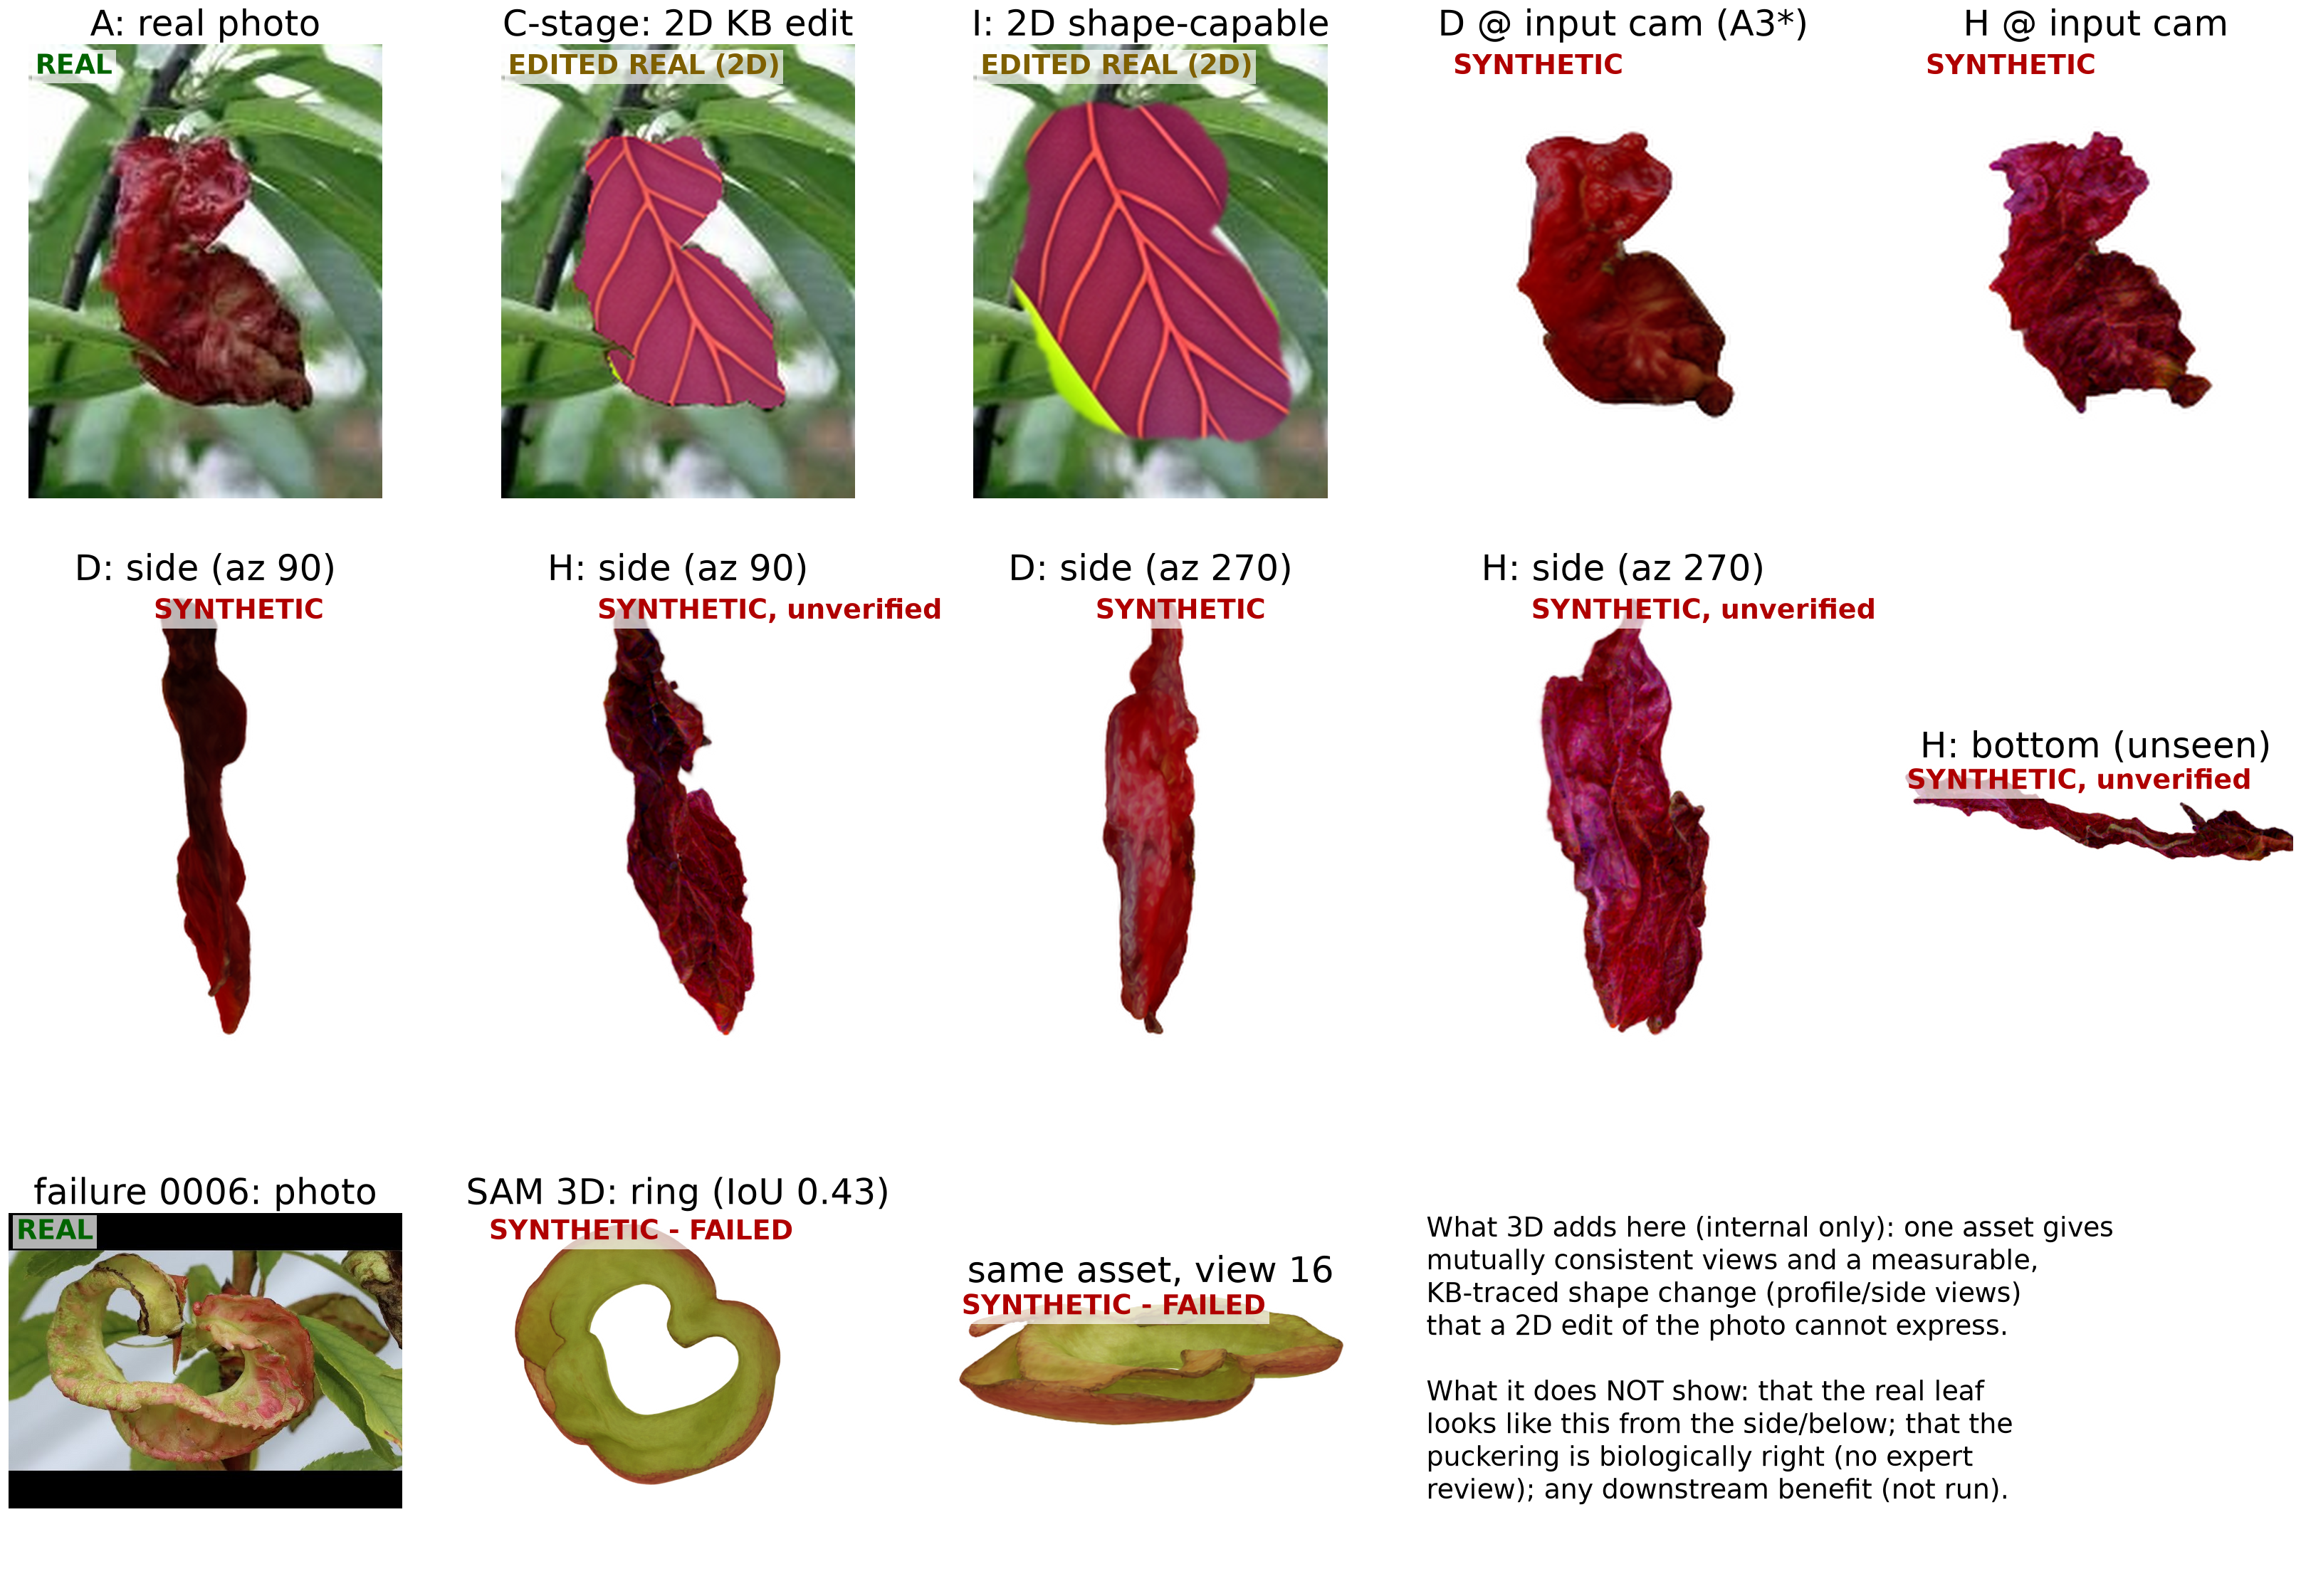
\includegraphics[width=\linewidth]{figs/fig10_added_value_Peach__Leaf_Curl__0087.png}\caption{Added value of the 3D asset vs 2D editing, with a reconstruction failure.}\end{figure}


\section{Decision (brief \S24) and next steps}
\paragraph{Outcome A (verified 3D reconstruction): not supported.} No independent reference (second view or 3D measurement) exists for any specimen. Input-view agreement after pose correction is a fit, not an accuracy measure.
\paragraph{Outcome B (knowledge-controlled 3D simulation): technical preconditions partly met; not established.} Three preconditions hold on the pilot:
\begin{itemize}
\item the KB-operator geometry editor gives coherent, regularised, KB-traceable shape change;
\item it realises more of the stage's KB geometric attributes than an equal-magnitude generic warp (small $n$, 2 classes, partly by construction);
\item one 3D asset is far more cross-view consistent than independent per-view 2D edits (internal consistency only).
\end{itemize}
Outcome B additionally requires \emph{biological validation}, which was not possible (no expert raters). The detectors are coarse; the depression detector is non-specific; on volumetric organs the outgrowth response is attenuated.
\paragraph{Outcome C (downstream augmentation): not tested.} The downstream classifier experiment (\S18) was not run. The Stage-5 gate requires a reliable controlled pilot first, and 15 assets cannot power a held-out comparison. At the measured $\approx$3.4 GPU-h per specimen for the full arm set, 250 assets need about 850 GPU-h locally. With only D, J and H per asset the figure is about 1 GPU-h per asset ($\approx$250 GPU-h, $\approx$5 days on two TITAN X).
\paragraph{Classification: Outcome D (no established advantage) for now.} Neither GaussianEditor nor the new pipeline has been shown to produce biologically valid disease geometry, and no advantage on real data has been measured. The evidence supports a narrower technical contribution: diagnosis and repair of the pipeline, plus a controllable, auditable KB$\to$geometry editing method with honest metrics.
\paragraph{Recommended next experiments, in priority order.}
\begin{enumerate}
\item \textbf{Blinded expert review} (2--3 plant pathologists). Rate stage-matched renders of D/J/H/K/F and 2D C-stage/I per specimen for symptom presence, stage correctness and implausible artefacts. This is the only way to move toward Outcome B.
\item \textbf{Operator coverage:} a directional \emph{roll} operator. Grape Leafroll's text specifies ``margins rolled under'', the clearest geometric KB claim in SAGE. Also calibrate outgrowth on synthetic volumes, and lesion-anchored (observed-spot) placement instead of random sites.
\item \textbf{Two-sided leaves:} SAM~3D leaves are single SH-0 sheets, so lower-surface symptoms (Tomato Leaf Mold, Squash Downy Mildew) cannot be represented. Duplicate the sheet with offset normals before any underside edit.
\item \textbf{Reference data for external validity:} even 20--30 specimens photographed from several views would turn every ``unverified'' label into a measurement. (Out of scope by current decision.)
\item \textbf{Downstream test (C)} only after 1--3: matched synthetic budget, leakage-safe SAGE test split, real-only vs +C-stage 2D vs +J/H 3D renders.
\end{enumerate}

\end{document}
